\documentclass{scrartcl}

% Tickz
\usepackage{tikz}
\usetikzlibrary{shapes}
\usetikzlibrary{arrows}
\usetikzlibrary{decorations.pathreplacing}
\usetikzlibrary{fit}
\usetikzlibrary{positioning}
\usetikzlibrary{shadows}
\usetikzlibrary{calc}
\usetikzlibrary{backgrounds}
\usetikzlibrary{matrix}

% Fonts
\usepackage{libertine} 
\usepackage[libertine]{newtxmath}
\renewcommand{\familydefault}{\sfdefault}
\usepackage[T1]{fontenc}
\usepackage[utf8]{inputenc}
\usepackage{courier}
\usepackage[scaled=.75]{beramono}

% Decorate key bindings and menu paths.
\usepackage{menukeys}

% Several figures in a figure.
\usepackage{subfig}

% Tables.
\usepackage{tabulary}
\usepackage{booktabs}

% Links.
\usepackage{hyperref}
\PassOptionsToPackage{hyphens}{url}
\usepackage[htt]{hyphenat}

% Colored links
\newcommand\coloredlink[1]{\textcolor{blue!75!black}{\underline{\smash{#1}}}}
\newcommand\wikilink[2]{\href{http://imagej.net/#1}{\coloredlink{#2}}}

% Epigraph
\usepackage{epigraph}

% Test math symbols.
\usepackage{textcomp}       

% Small images in text (for e.g. small icon).
\newcommand*{\smallimg}[1]{%
  \raisebox{-.1\baselineskip}{%
    \includegraphics[
      height=0.7\baselineskip,
      width=\baselineskip,
      keepaspectratio,
    ]{figures/#1}%
  }%
}

% Properly hyphen TrackMate & TrackScheme & friends
\newcommand\TrackScheme[0]{Track\-Scheme\ }
\newcommand\TrackMate[0]{Track\-Mate\ }
\newcommand{\bdv}{BigDataViewer\ }
\newcommand{\Bdv}{BigDataViewer\ }
\newcommand{\Ie}{\textit{I.e.{}}\ }
\newcommand{\Eg}{\textit{E.g.{}}\ }
\newcommand{\Cf}{\textit{Cf.{}}\ }
\newcommand{\ie}{\textit{i.e.{}}\ }
\newcommand{\eg}{\textit{e.g.{}}\ }
\newcommand{\cf}{\textit{cf.{}}\ }
\newcommand{\etc}{\textit{etc}\ }
\newcommand{\etal}{\emph{et~al.}}

% Making 1.5 spaced lines
\usepackage{setspace}
\onehalfspacing

% Syntax highlighting
\usepackage{minted}
\setminted{fontsize=\small, baselinestretch=1}

% More space between paragraphs and indent.
\setlength{\parskip}{6pt}
\setlength\parindent{24pt}

% Figure caption with special fonts.
\usepackage[font=small,labelfont=bf,format=plain]{caption}

% Smaller margins. Paper is expensive and we write in big characters.
\usepackage[margin=1in]{geometry}


%---------------------------------------------------------------------------------
% Contents
%---------------------------------------------------------------------------------

\begin{document}

\begin{titlepage}

\begin{tikzpicture}[overlay,remember picture]
\draw [line width=1.0pt,rounded corners=10pt,]
    ($ (current page.north west) + (2cm, -2cm) $)
    rectangle
    ($ (current page.south east) + (-2cm, 2cm) $);       
\end{tikzpicture}

\begin{center}
        
    \vfill
    
	{\fontsize{60}{70}\selectfont \textbf{Mastodon}}
	{\fontsize{40}{50}\selectfont \textbf{documentation}} \\ 
	\protect{
\includegraphics[width=12cm]{figures/Mastodon-logo_jy-01.png}}
    
    \LARGE{Tobias Pietzsch \& Jean-Yves Tinevez} \\
    \LARGE{\today}
    
    \vfill
    
\includegraphics[width=4cm]{figures/Pasteur-logo-medium.png}
    \hfill
    
\includegraphics[width=4cm]{figures/MPICBG_logo_bw.png}%



\end{center}
% \thispagestyle{empty}

\end{titlepage}

\newpage
This document constitutes the \wikilink{Mastodon}{Mastodon} documentation. 
It is divided in four parts, that group sections by interest.
\begin{myitemize}
	
	\item The first part contains three tutorials, aimed at end-users and focused on cell tracking.
	They are meant to guide users with the Mastodon software and cover three applications of cell tracking Mastodon:
	\begin{myitemize}
		\item automated cell or particle tracking;
		\item manual curation and correction of tracking results;
		\item manual and semi-automatic tracking.
	\end{myitemize}
	
	\item The second part contains technical information. ...
	
	\item The third part is aimed at advanced users, ...
	
	\item The last part is made of tutorials aimed at Java developers ...
	
\end{myitemize}


\newpage
\tableofcontents

% Introduction and generalities about Mastodon.
\newpage
\section{Getting started with Mastodon. Automated tracking.}
\label{sec:GettingStarted}

This tutorial is the starting point for new Mastodon users. 
It will walk you through basic operations in Mastodon, opening a dataset and creating a Mastodon project, automatically detect cells and link them, and show you how to use the main views of Mastodon.
We don't go into details, and will revisit the features we survey here later.

\subsection{The image data.}

\subsubsection{Exporting your image to \Bdv file format.}

Mastodon uses \wikilink{BigDataViewer}{\Bdv} (BDV) files as input images.
You need to prepare your images so that they can be opened in the \bdv.

BDV files are used more and more by several software projects in the Fiji ecosystem and beyond. 
This tutorial focuses on Mastodon not on BDV, however we will take a very small detour to explain what makes it fit and how to turn your images into this format. 
If you know already, you can skip this part, because we simply recapitulate what is being explained in the original \Bdv publication~\cite{bdv}.

For this tutorial we will use a ready-made dataset, in the adequate format, but it is a good idea to know how to export or create an image in such a format.
We lazily rely on the excellent \bdv documentation and point directly to the \bdv instructions to prepare your images, \eg depending on whether
\begin{itemize}
	\item they are \wikilink{BigDataViewer\#Exporting_from_ImageJ_Stacks}{opened as an ImageJ stack}, or
	\item they come from a \wikilink{BigDataViewer\#Integration_with_Fiji.27s_SPIMage_Processing_Tools}{SPIM processing pipeline}, or
	\item they come from the \wikilink{BigStitcher}{BigStitcher} plugin~\cite{BigStitcher}, \etc.
\end{itemize}

Once you have prepared your images for opening in the \bdv, you should have a \texttt{.xml} file and a possibly very large \texttt{.h5} file on your computer. The \texttt{.xml} file must be the output of the \bdv data preparation. It should start with the following lines:

\begin{lstlisting}[language=XML]
<?xml version="1.0" encoding="UTF-8"?>
<SpimData version="0.2">
  <BasePath type="relative">.</BasePath>
  <SequenceDescription>
    <ImageLoader format="bdv.hdf5">
      <hdf5 type="relative">datasethdf5.h5</hdf5>
...
\end{lstlisting}


\subsubsection{Key advantages of the \Bdv file format.}
\label{sec:BDVAdvantages}

The BDV file format solves mainly two challenges in image visualization and analysis, that arise with modern microscopy, namely:
\begin{itemize}
    
    \item Modern microscopes can generate images that are very large in size. Much larger that what can be fitted in RAM, even with the increase in computer power. It is now common to find single movies acquired on SPIM microscopes that are several TBs in size. Computers with several TBs of RAM are not so common.
    
    \item Multiple views of the same sample can be acquired, and they need to be visualized in the same viewer. The first use case is also the multi-view images generated by SPIM microscopes, but we can also think of correlative light-electron microscopy.
    
\end{itemize}

If we focus on the first challenge, you see that we need to stream the image data directly from the disk, instead of fully loading it into RAM. 
But at the same time, we need a tool that allows for interactive browsing of the data. 
The view must be responsive to the user input, and not block when it has to load the data from the file. 
The BDV file format offers a clever file format design that does this, coupled to a specialized viewer.
The image data are stored in small chunks corresponding to a neighborhood. As the viewer shows a slice through the image, the required chunks are loaded on demand and cached.
All the chunks are organized in a HDF5 file, which is like a file-system in a file\footnote{\href{https://en.wikipedia.org/wiki/Hierarchical_Data_Format}{\coloredlink{Hierarchical Data Format} on Wikipedia.}}, and accessing single chunks is fast with current computer hardware.
On top of this, the image is also stored as a multi-scale pyramid\footnote{\href{https://en.wikipedia.org/wiki/Pyramid_(image_processing)}{\coloredlink{Multi-scale pyramid} on Wikipedia.}}, to speed-up zooming and unzooming (Figure~\ref{fig:BDVchunks}).
The BDV display component exploits this file format in a clever way, and ensures that the view still answers to user interactions (mouse pan, zoom, clicks \etc) even if the chunks are not full loaded.

\begin{figure}
    \centering
    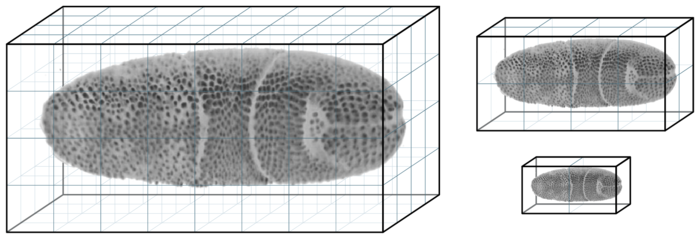
\includegraphics[width=0.6\textwidth]{figures/BdvTikz-pyramidblocks.png}
    \caption{Illustration of the BDV file format storage strategy. The image is stored over several resolution levels (multi-scale pyramid) and in chunks.}
    \label{fig:BDVchunks}
\end{figure}

There are several implementations of this strategy, for instance in Imaris\footnote{\href{http://open.bitplane.com/Default.aspx?tabid=268}{\coloredlink{IMARIS 5.5 File Format Description (IMS).}}} and with the new file format N5\footnote{\href{https://github.com/saalfeldlab/n5}{\coloredlink{N5 API on GitHub.}}} proposed by the Saalfeld lab.
Some of them are inter-compatible.
We will pick the BDV file format all along this document. 
The \Bdv has proved its value and impact on our field.
For instance our previous work on cell lineaging in large images, \wikilink{MaMuT}{MaMuT}, is based on BDV~\cite{MaMuT}.



\subsubsection{The tutorial dataset.}

Mastodon was created specially because we needed to harness very big, multi-view images. We wanted to generate  comprehensive lineages and follow a large number of cells over a very long time.
This accumulation of inflated words is tied to the very large  - in objective disk space  occupation - images we deal with using modern microscopy tools. 
Such datasets might not be optimal for a first contact with Mastodon.
So just for this tutorial we will use a smaller dataset.
It is a small region cut into a movie following the development of a drosophila embryo, acquired by William Lemon in Patrick Keller lab (HHMI, Janelia Farm).
This was created from the example dataset released with the TGMM software~\cite{TGMMpaper}.
You can find it on Zenodo\footnote{\href{https://zenodo.org/record/3336346}{\coloredlink{https://zenodo.org/record/3336346}}} there: \href{https://doi.org/10.5281/zenodo.3336346}{
\includegraphics[height=1.5\fontcharht\font`\B]{figures/zenodo3336346.png}}

It is a zip file that contains 3 files:
\begin{lstlisting}[language=sh]
    14M  datasethdf5.h5
   2.7K  datasethdf5.settings.xml
   8.7K  datasethdf5.xml
\end{lstlisting}

The \texttt{.h5} file is the HDF5 file mentioned above, that contains the image data itself.
The \texttt{data\-sethdf5.xml} is a text file following the XML convention, specific to the BDV file format, that contains information about the the image data and metadata. 
When we want to open a BDV file, we point the reader to this file.
The \texttt{datasethdf5.settings.xml} is an optional file that stores user display parameters, such as channel colors, min and max display value, as well as bookmarks in the data. 
We refer you to the \wikilink{BigDataViewer\#Loading_and_Saving_Settings}{BDV documentation} about this file.
Mastodon uses this settings file to store that same information.

If you open this data in the \Bdv (in Fiji in the \menu{Plugins > BigDataViewer > Open XML/HDF5} menu), you should see something like in figure~\ref{fig:OpeningImage}. 
There is about 70 cells in each of the 30 time-points, arranged in a layer at the top of the sample. 
The deeper part of the sample (low Z coordinates) has some hazy, diffuse signal from which we cannot individualize cells.
As time progresses, the cells move towards the middle part and bottom (high Y coordinates) part of the image, and some of them move deeper in Z, initiating gastrulation.

The goal of this short tutorial is to track all these cells in Mastodon.

\begin{figure}
     \centering
         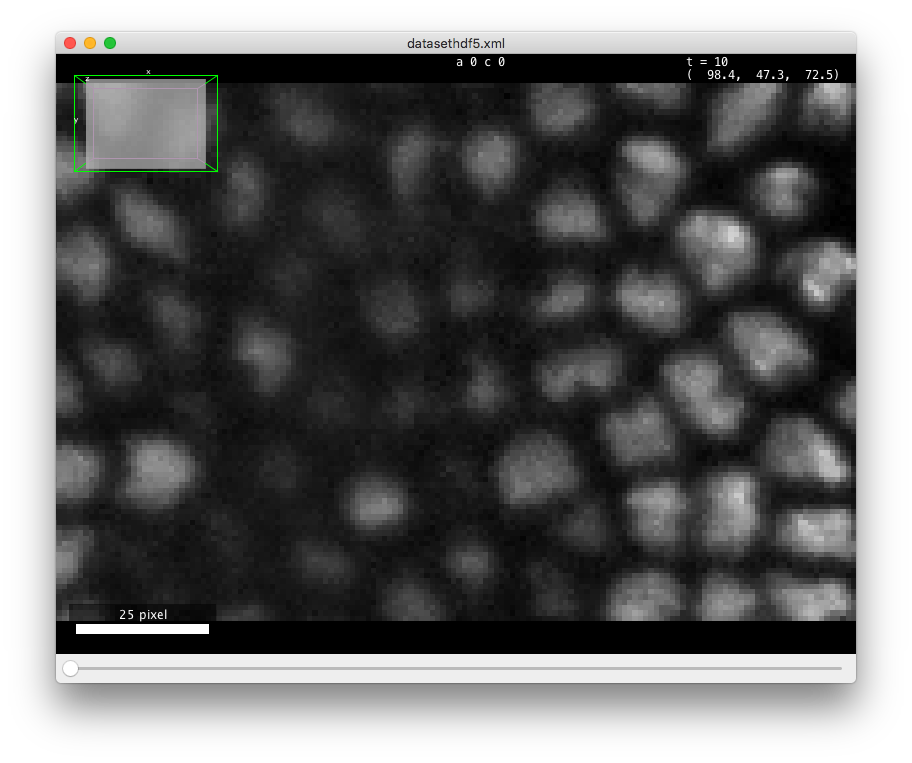
\includegraphics[width=0.3\textwidth]{figures/BDV-imageXY.png}
         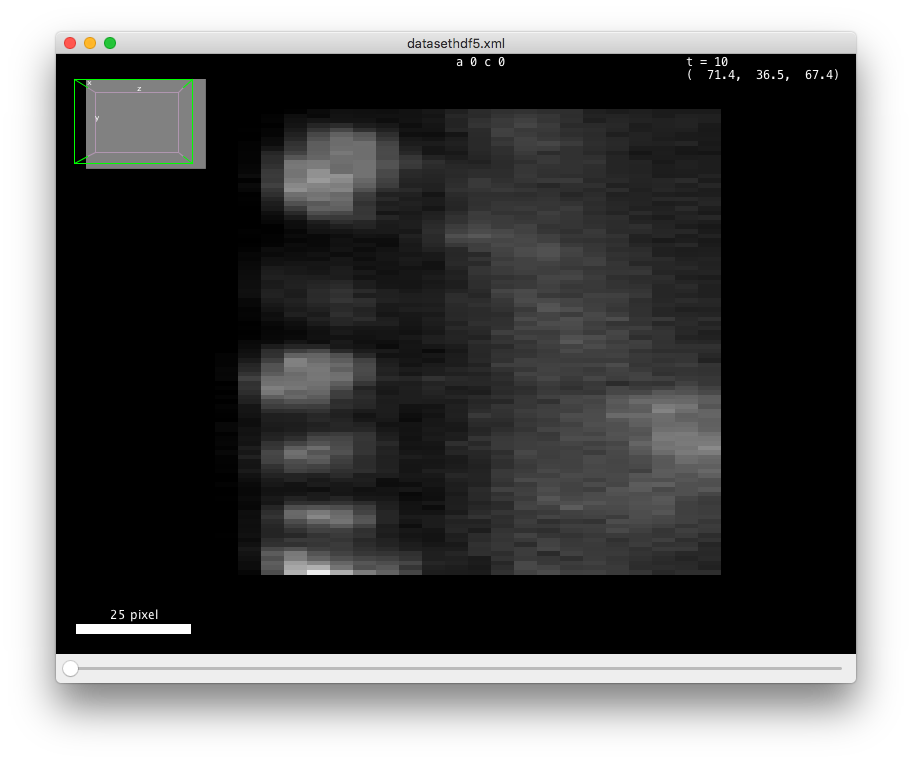
\includegraphics[width=0.3\textwidth]{figures/BDV-imageXZ.png}
         \caption{The tutorial dataset opened in \Bdv, seen along XY (left) and XZ (right)}
     \label{fig:OpeningImage}
\end{figure}  




\subsection{Getting Mastodon.}

As of today, Mastodon is available as a preview. We are still working on adding and validating features.
Nonetheless the preview has everything we need to track these cells.
Also, Mastodon is independent of ImageJ or Fiji, it can operate as a standalone software. 
However we currently distribute it via Fiji, because the updater and the dependency management are so convenient. 
So the first thing to do is to grab Fiji\footnote{\href{http://fiji.sc/}{\coloredlink{http://fiji.sc/}}}, if you do not have it already.

Then launch the \wikilink{Updater}{Fiji updater} and once your Fiji is up to date, click on the \texttt{Manage update site} button.
We will add the \wikilink{Following_an_update_site}{add the Mastodon update site}.
You should find the Mastodon preview site in the list. 
Select it, update Fiji and restart it. 
After restarting, you should find the command \menu{Plugins > Mastodon (preview)} at the bottom of the menu.

\begin{center}
    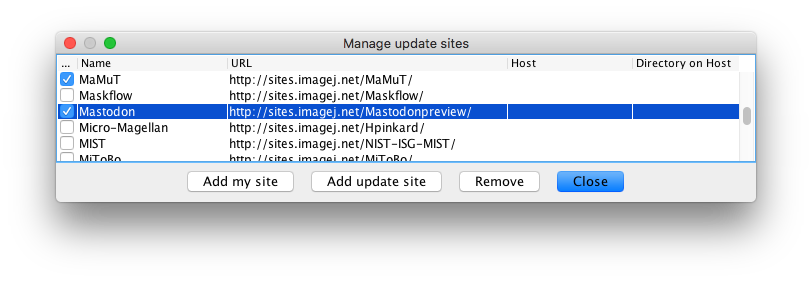
\includegraphics[width=0.7\textwidth]{figures/Mastodon_UpdateSite.png}
\end{center}

\subsection{Creating a new Mastodon project.}

After launching the command, this plain, sober window appears.
\begin{figure}[!htbp]
    \centering
    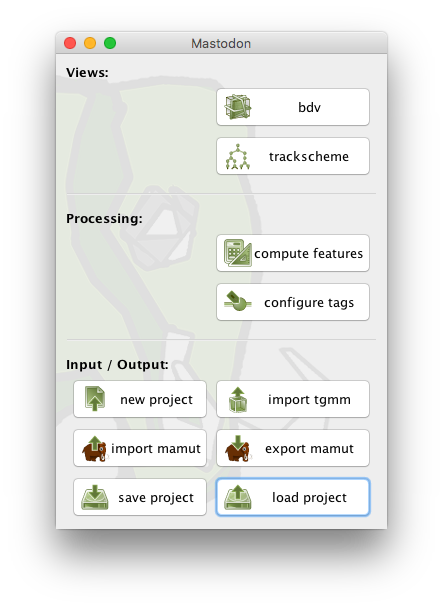
\includegraphics[width=0.3\textwidth]{figures/Mastodon_MainWindow.png}
    \caption{The main window of Mastodon.}
    \label{fig:MastodonMainWindow}
\end{figure}

Click on \menu{new project}, and browse to the \texttt{datasethdf5.xml} file of the XML/HDF5 file pair of the tutorial dataset.
All the buttons that were grayed out should be now enabled. 
Click on the \menu{bdv} button.
A BDV window should appear and if it does everything is right.
\begin{center}
         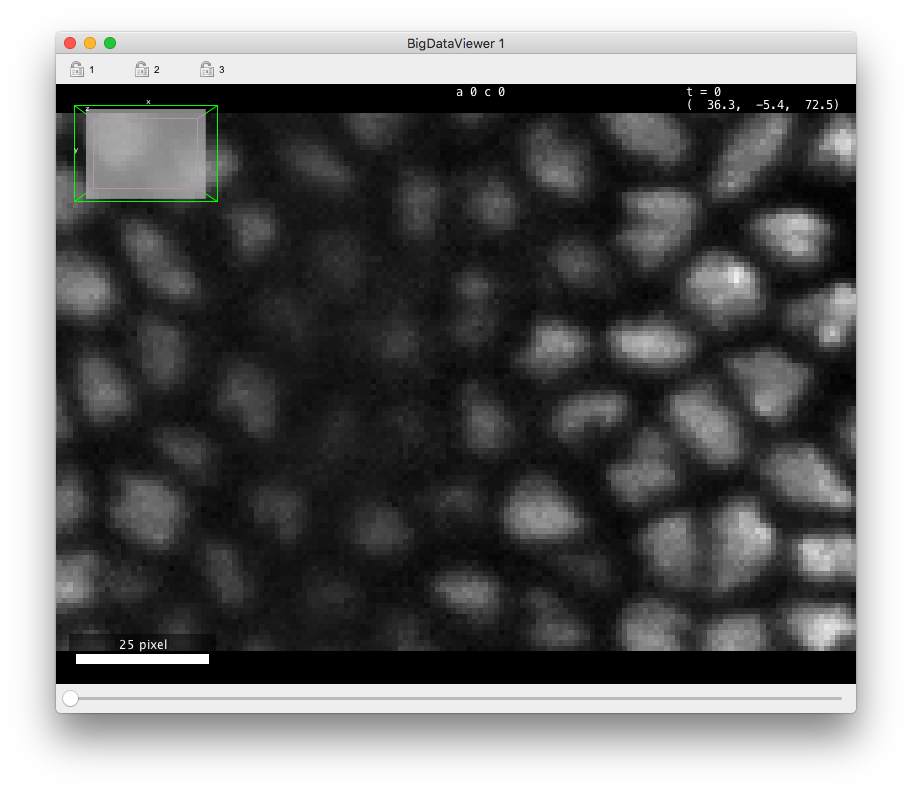
\includegraphics[width=0.4\textwidth]{figures/Mastodon_BDV.png}
\end{center}

It is almost a regular BDV window and if you already know who to use it and the key bindings you should find your marks quickly.
The BDV view displays a \textit{slice} of the image through arbitrary orientation. 
Below we give the commands and key-bindings for navigation in a Mastodon-BDV window. 
They are indeed close to what is found in the standard \Bdv but some changes. 
\textbf{Please note:} You can reconfigure almost everything in Mastodon, as we will see later, including key-bindings.
In this tutorial and the next ones, the key-bindings we present are for the \texttt{Default} configuration.
In the table~\ref{tab:MastodonBDVNavigationKeys} page~\pageref{tab:MastodonBDVNavigationKeys} you will find the key bindings to navigate through the image data.

\begin{table}[!htbp]
    \centering
    
    \caption{Default navigation key-bindings for Mastodon-BDV views.}

    \begin{tabulary}{\textwidth}{L|J}
    
    \toprule
    \textbf{Action}                 & \textbf{Key}              
    \\ \midrule
    
    \multicolumn{2}{c}{\textit{View.}}
    \\ \midrule
    
    Move in X \& Y.                 & \keys{Right-click} and \keys{Drag}
    \\ \midrule
    
    Move in Z.                      & \keys{Mouse-wheel}. Press and hold \keys{\shift} to move faster, \keys{\ctrl} to move slower.
    \\ \midrule
    
    Align view with X / Y / Z axes. &  
    \begin{minipage}[t]{0.7\textwidth}
    \begin{itemize}
        \item  Align with XY plane: \keys{\shift+Z}
        \item Align with YZ plane: \keys{\shift+X}
        \item Align with XZ plane: \keys{\shift+C} or \keys{\shift+Y} 
    \end{itemize}
    The view will rotate around the location you clicked.
    \end{minipage}
    
    \\ \midrule
    
    Zoom / Unzoom.                  & \keys{\ctrl+\shift+Mouse-wheel} or \keys{\cmd+Mouse-wheel}. The view will zoom and unzoom around the mouse location.
    \\ \midrule

    \multicolumn{2}{c}{\textit{Time-points.}}
    \\ \midrule
    
    Next time-point.                & \keys{]} or \keys{M}
    \\ \midrule
    
    Previous time-point.            & \keys{[} or \keys{N}                                                                                     
    \\ \midrule

    \multicolumn{2}{c}{\textit{Bookmarks.}}
    \\ \midrule

    Store a bookmark.               & \keys{\shift+B} then press any key to store a bookmark with this key as name. A bookmark stores the position, zoom and orientation in the view but not the time-point. Bookmarks are saved in display settings file.
    \\ \midrule
    
    Recall a bookmark.              & Press \keys{B} then the key of the bookmark.
    \\ \midrule  
    
    Recall a bookmark orientation.  & Press \keys{O} then the key of the bookmark. Only the orientation of the bookmark will be restored.
    \\ \midrule
    
    \multicolumn{2}{c}{\textit{Image display.}}
    \\ \midrule
    
    Select source 1, 2 \ldots         & Press \keys{1} / \keys{2} \ldots
    \\ \midrule
    
    Brightness and color dialog.    & Press \keys{S}. In this dialog you can adjust the min \& max for each source, select to what sources these min \& max apply and pick a color for each source.
    \\ \midrule
    
    Toggle fused mode.              & Press \keys{F}. In fused mode, several sources are overlaid. Press \keys{\shift+1} / \keys{\shift+2} \ldots to add / remove the source to the view. In single-source mode, only one source is shown.
    \\ \midrule
    
    Visibility and grouping dialog.     & Press \keys{F6}. In this dialog you can define what sources are visible in fused mode, and define groups of sources for use in the grouping mode.
    \\ \midrule
    
    Save / load display settings.       & \keys{F11} / \keys{F12}. This will create a \texttt{XYZ\_settings.xml} file in which the display settings will be saved.
    \\ \bottomrule

\end{tabulary}


    \label{tab:MastodonBDVNavigationKeys}
    \vspace{-10pt}

\end{table}

Now you want to save the project. 
Go back to the main window, and click on the \menu{save project} button.
This will create a single file, called for instance \texttt{drosophila\_crop.mastodon} file. 
This file is actually a zip file that contains the tracks and \textit{links} to the image data.
The image data is kept separate from the Mastodon file, which allows for using it with another software, independently. 
So if you want to transfer or move a full Mastodon project, you need to take the \texttt{.mastodon} file and all the \texttt{.xml} and \texttt{.h5} files from the \Bdv dataset.

Next time you want to open this project, just click on the \menu{load project} button and point the file browser to the \texttt{.mastodon} file.
The image data will be loaded along with the lineages.



\subsection{Detecting cells.}
\label{sec:DetectingCells}

\begin{figure}
    \centering
     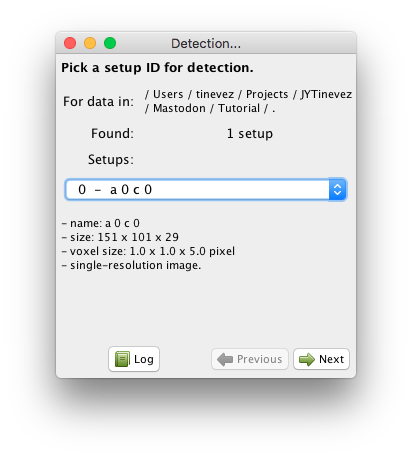
\includegraphics[width=0.4\textwidth]{figures/Mastodon_DetectionWizard_01.png}
     \caption{First panel of the detection wizard.}
     \label{fig:DetectionWizardFirstPanel}
\end{figure}

We want to track automatically all the cells in this dataset, and the first step is therefore to detect them.
Mastodon ships a wizard to perform cell detection. 
It is very much inspired by the \wikilink{TrackMate}{TrackMate} GUI, and if you know this software you will find your marks here.
Also, the algorithms are very close to what was in TrackMate~\cite{TrackMate}, but they have been heavily optimized for Mastodon.

The detection wizard can be launched from the \menu{Plugins > Tracking > Detection...} menu item. 
You should have a window like the one depicted in Figure~\ref{fig:DetectionWizardFirstPanel}.

Like for TrackMate, the automated tracking user interface uses \textit{wizards} to enter parameters, select algorithms, \textit{etc.}
You can navigate back and forth with the \menu{\smallimg{arrow_right.png} Next} and  \menu{\smallimg{arrow_left.png} Previous} buttons. 
The \menu{\smallimg{book.png} Log} button will bring an independent panel where all the activity in the wizard are logged as text. 

This first panel allows for selecting the target \textit{source} on which the detection will be run. 
Since we use the \bdv for images, a channel or a view is stored and displayed as a source. 
A source can have multiple resolutions stored, as explain in paragraph~\ref{sec:BDVAdvantages}, but for the data used in this tutorial this is not the case. The sources are nicknamed 'setups' in this panel.
They are numbered from 0 and can be selected from the drop-down list. 
Below the list we try to display the metadata we could retrieve from the \bdv file.
Just pick the first and only channel, and click \menu{\smallimg{arrow_right.png} Next}.

You can now choose to operate only on a rectangular ROI in the image. 
If you check the \textbf{Process only a ROI} button, new controls appear in the panel, and a ROI is drawn into an open BDV view (a new one is created if one is not opened).
The ROI is painted as a wire-frame box, green for vertices that point towards the camera from the displayed slice, and purple for vertices that points away from the camera, below the displayed slice.
The intersection of the ROI box with the displayed slice is painted with a purple semi-transparent overlay, with a white dotted line as borders.
You can control the ROI bounds with the controls in the panel, or by directly dragging the ROI corners in the BDV view.
Time bounds can also be set this way. In our case we want to segment the full image over all time-points, so leave the \textbf{Process only a ROI} button unchecked.

You cannot have non-rectangular ROIs in Mastodon. Nonetheless they are super useful as is. 
You can for instance combine several detection steps using different parameters in different region of your image. Or different time interval.

\begin{center}
     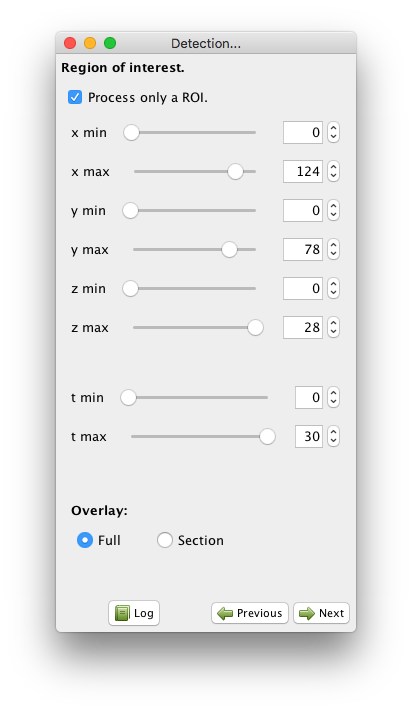
\includegraphics[height=0.25\textheight]{figures/Mastodon_ROIpanel.png}
     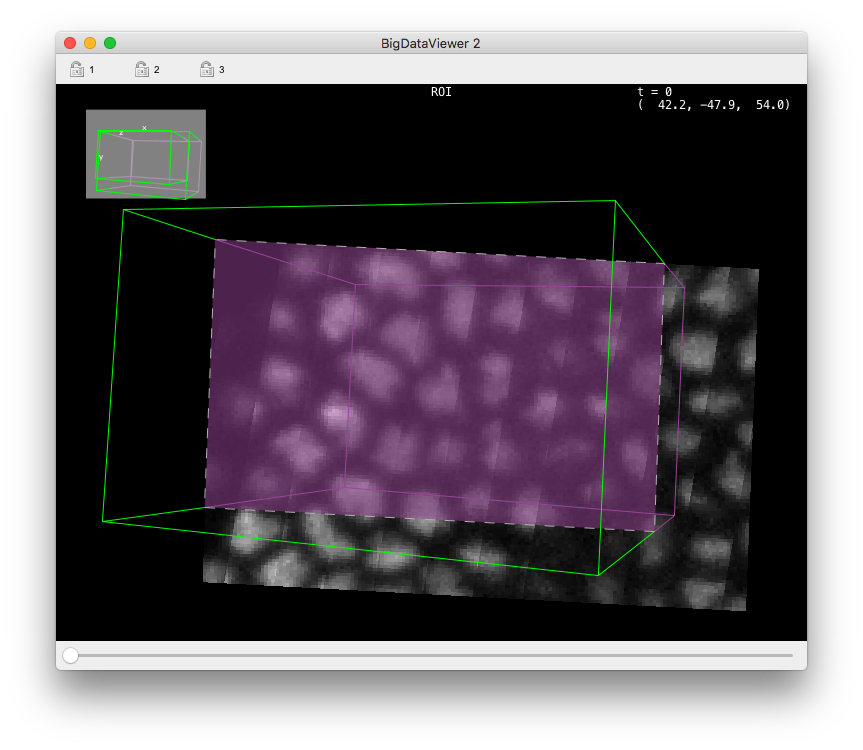
\includegraphics[height=0.25\textheight]{figures/Mastodon_ROIBDV.png}
\end{center}

The next panel lets you choose the detector you want to use.
In vanilla Mastodon, three detectors are available.
Right now, we will use the default one, the \textbf{DoG detector}, which should be good enough for most cases.
DoG means 'difference-of-Gaussians'.
It is an efficient approximation of the LoG ('Laplacian of Gaussian') filter, and there is also a detector in Mastodon based on the latter.

These detectors excel at finding roundish structures in the image that are bright over a dark background.
The structures must have a shape somewhat close to a sphere, but they can accommodate a lot of variability.
As a rule of thumb, if you can define rough estimate of the radius of these structures, they are eligible to be picked up by our detectors. 
This also implies that in Mastodon, we cannot segment complex shapes, or object labeled by their contour (\textit{e.g.} cell membranes), or even exploit these shapes to have an accurate measurements of the volume. 
This is an important limitation of Mastodon.

For now, select the \textbf{DoG detector} and click \menu{\smallimg{arrow_right.png} Next}.
\label{sec:DetectionCellsDoGDetector}

Here is briefly  how it works.
The LoG detector, and its approximation the DoG detector, is the best detector for blob-like particles in the presence of noise~\cite{Sage2005}. 
It is based on applying a Laplacian of Gaussian (LoG) filter on the image and looking for local maxima. The result is obtained by summing the second order spatial derivatives of the gaussian- filtered image, and normalizing for scale.
Local maxima in the filtered image yields spot detections. 
Each detected spot is assigned a \textbf{quality} value, that is obtained by taking the intensity value in the LoG filtered image at the location of the spot.
So by properties of the LoG filter, this quality value is larger for :
\begin{itemize}
    \item bright spots;
    \item spots which diameter is close to the specified diameter.
\end{itemize}

The DoG detector requires only two parameters: the estimated diameter of the object we want to detect, and a threshold on the quality value, that will help separating spurious detections from real ones. 
The panel you are presented let you specify these parameters, and preview the resulting detection.
Try with 10 pixels for \textbf{Estimated diameter} and 0 for the \textbf{Quality threshold}.
The click on the \menu{\smallimg{led-icon-eye-green.png} Preview} button.
A preview panel should open shortly, showing detection results on the current frame (Figure~\ref{fig:PreviewDetection}).

\begin{figure}
    \centering
         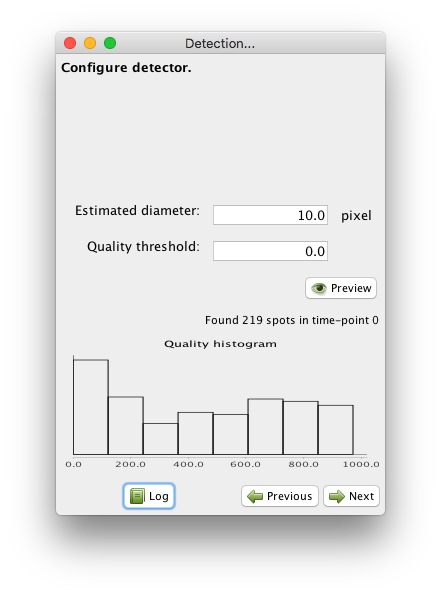
\includegraphics[height=0.25\textheight]{figures/Mastodon_DoGconfig1.png}
         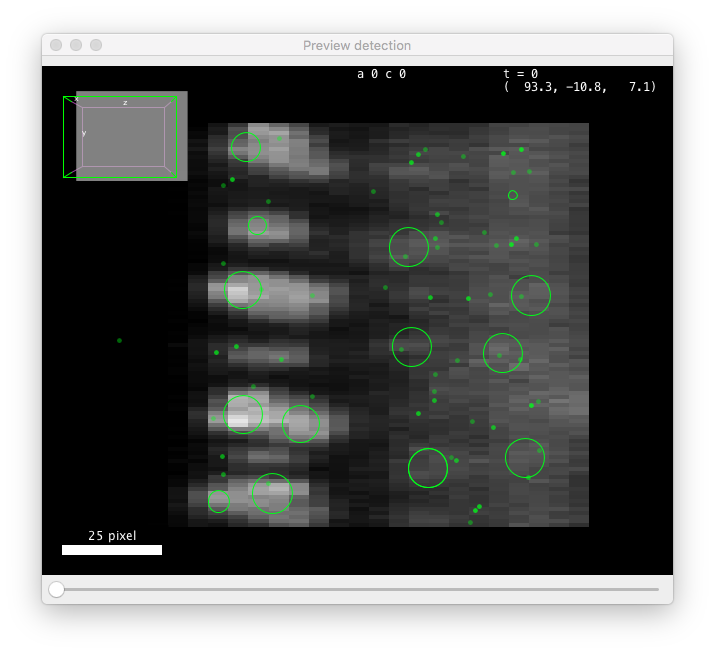
\includegraphics[height=0.25\textheight]{figures/Mastodon_DoGconfig2.png}
    \caption{Previewing detection results.}
    \label{fig:PreviewDetection}
\end{figure}

These values are close but not quite.
You can see that the diameter value is too small to properly grasps the elongated shape of the cells along Z (the BDV view on the left panel above is rotated to show a YZ plane). 
Also the threshold value is too low, and some spurious detections are found below the epithelium.
These spots have a low quality, that manifests as a peak at low value in the quality histogram displayed on the configuration panel.
From the shape of the histogram, we can infer that a threshold value around 100 should work.
However we also need to change the diameter parameter, which will change the range of quality values.
After trial and errors, values around 15 pixels for the diameter and 400 for the threshold seem to work.

Note that you can run the preview on any frame.
You just have to move the time slider on the preview window.
Once you are happy with the parameters, click on the \menu{\smallimg{arrow_right.png} Next} button.
All the frames specified in the ROI (if any) will be processed. 
In our case detection should conclude quickly and the following panel should appear:

We now have more than 1000 cells detected and this concludes the detection step (Figure~\ref{fig:DetectionResults}).
Click on the \menu{\smallimg{accept-icon.png} Finish} button, and the wizard will disappear.

\begin{figure}
    \centering
    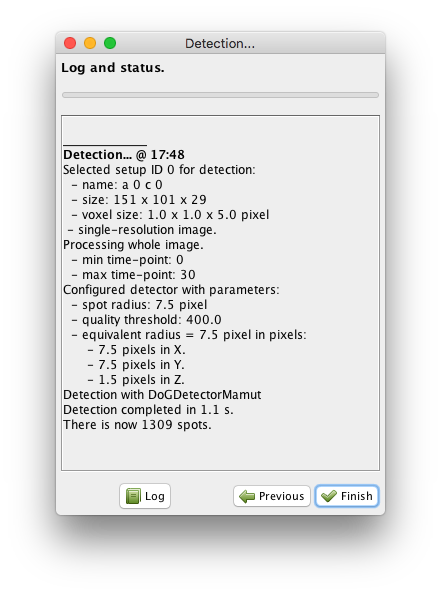
\includegraphics[height=0.40\textwidth, trim=0.5cm 0.5cm .5cm .5cm, clip]{figures/Mastodon_DetectionResuts.png}
    \caption{Detection results.}
    \label{fig:DetectionResults}
\end{figure}

If you have complex images mixing several size of objects, or detection parameters that work for one part of the movie but not for another one, you could restart a new detection now, selecting for instance other parts of the movie with the ROI.
You can do this and more, but for this kind of approach, the \textbf{Advanced DoG detector} offers more configuration capabilities, that will review later.



\subsection{Linking cells.}

What we just did is the detection step. 
It yields one Mastodon spot per cell, but the notion of cell identity propagated over time is missing yet.
The particle linking step just does that.
A particle linking or tracking algorithm accepts a collection of spots, ordered by frames (time-points), and tries to link each spot to the next spot(s) in the next frame or so. 
All the spots you can reach by starting from one spot and navigating across links build a \textit{track}, and in our case it represents one cell (or any other object) followed over time. 
In most cases there is one spot per frame for a track, meaning that that a spot has at most one incoming link (spot from previous frame) and one outgoing kink (spot in next frame). 
But some algorithms can accommodate \textit{e.g.} dividing cells (2 outgoing links for the mother cell going to the two daughter cells) and merging events. There is a vast literature behind tracking algorithms, and it is an active domain of Research. A relatively recent paper compare implementation and list some pros and pitfalls of many of them~\cite{Chenouard2014}.

\subsubsection{Selecting target spots for linking.}

\begin{figure}
    \centering
    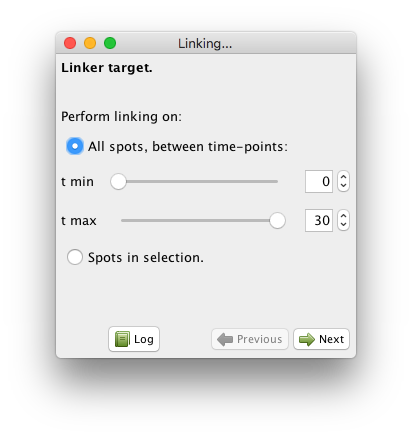
\includegraphics[height=0.3\textwidth,trim=0.5cm .5cm .5cm .5cm,clip]{figures/Mastodon_LinkingWizard_01.png}
    \caption{The first panel of the linking wizard.}
    \label{fig:LinkingWizardFirstPanel}
\end{figure}

Like for the detection step, linking in Mastodon happens in a wizard.
And also like for detection, the linking algorithms currently available in Mastodon are adapted from TrackMate. 
Launch the wizard from the GUI, with the \menu{Plugins > Tracking > Linking...} menu item. 
The first panel you are shown lets you select what spots to include in linking (Figure~\ref{fig:LinkingWizardFirstPanel}). 
There are two modes:
\begin{itemize}
    \item Either you take all the spots between a start and and end frame. By default, all frames are selected.
    \item Either you specify you want to link only the spots that are in the selection. 
    This mode offers a lot of flexibility when facing complicated cases. 
    It is best use along with the selection creator, that we will introduce later in this manual.
\end{itemize}
For now, just leave the parameters as they are, which will include all spots in the linking process, and click next.
You can now choose between several linking algorithms. 

\subsubsection{Available linking algorithms in Mastodon.}

In Mastodon, they fall mainly in two categories.

The first two LAP trackers are based on the \textbf{Linear Assignment Problem (LAP) framework}, first developed by Jaqaman \textit{et al.}~\cite{Jaqaman2008}, with important differences from the original paper described elsewhere~\cite{TrackMate}. 
We focused on this method for it gives us a lot of flexibility and it can be configured easily to handle many cases. 
You can tune it to allow splitting events, where a track splits in two, for instance following a cell that encounters mitosis. 
Merging events are handled too in the same way. More importantly are gap-closing events, where a spot disappear for one frame (because it moves out of focus, because detection failed, ...) but the track manages to recuperates and connect with reappearing spots later.

In Mastodon the LAP algorithms exists in two flavors: a simple one and a not simple one. There are again the same, but the simple ones propose fewer configuration options and a thus more concise configuration panel. In short:
\begin{itemize}
    \item The simple one only allows to deal with gap-closing events, and prevent splitting and merging events to be detected. Also, the costs to link two spots are computed solely based on their respective distance.
    
    \item The not simple one allows to detect any kind of event, so if you need to build tracks that are splitting or merging, you must go for this one. If you want to forbid the detection of gap-closing events, you want to use it as well. Also, you can alter the cost calculation to disfavor the linking of spots that have very different feature values.
\end{itemize}

The third tracker is called \textbf{Linear motion Kalman linker}.
It can deal specifically with linear motion, or particles moving with a roughly constant velocity.
This velocity does not need to be the same for all particles. 
It relies on the Kalman filter\footnote{\href{https://en.wikipedia.org/wiki/Kalman_filter}{\coloredlink{Kalman filter on Wikipedia.}}} to predict the most probable position of a particle undergoing (quasi) constant velocity movement.

\subsubsection{How to pick the right linking algorithm?}

The right choice of a particle linking algorithm is conditioned by the expected motion of the object you track.
As a rule of thumb, you can make a decision following these simple rules:
\begin{itemize}
    
    \item If the objects you track are transported by an active process and have a motion for which the velocity vector changes slowly, then pick the  \textbf{Linear motion Kalman linker}.
    
    \item If the object motion is random (like in Brownian motion) or unknown, pick on the LAP linker. If the objects you track do not divide, nor merge, pick the \textbf{Simple LAP linker}.
    
    \item If the objects divide or merge, or if you want to specify linking costs based on numerical features (like spot mean intensity), then pick the \textbf{LAP linker}.
    
\end{itemize}
In our case, we need the \textbf{Simple LAP linker}. Select it and click \menu{\smallimg{arrow_right.png} Next}.

\subsubsection{Running the Simple LAP linker.}

This linker only requires the specification of three parameters.

The first one is the \textbf{Max linking distance} during frame-to-frame linking. 
It is the distance beyond which linking a spot to another one in the next frame will be forbidden. 
For instance, if you know that your objects move by at most 5~{\textmu}m from one frame to the next, pick a value slightly larger, for instance 6~{\textmu}m.
Distances are expressed in whatever physical units the BDV dataset specified.
In our case it is pixels. 

\begin{center}
    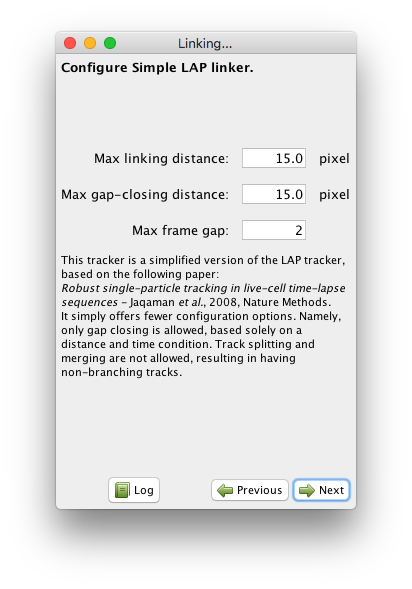
\includegraphics[height=0.25\textheight,trim=0.5cm .5cm .5cm .5cm,clip]{figures/Mastodon_LinkingWizard_03.png}
\end{center}

In practical cases, it can happen that the detection step might miss an object in some frames, then detect again later.
These gaps will result in generating several small tracks for a single objects, which is one of the main course of spurious results when analyzing tracks. 
The simple LAP linker can bridge over missed detections.
It does so by inspecting small tracks that results from frame-to-frame linking, and tries to connect the end of one with the beginning of another one.
The last two parameters of the linker specifies how they are bridged. 
The \textbf{Max gap-closing distance} specifies how far can we look for candidates when we try to bridge the end of a track with the beginning of another one.
The \textbf{Max frame gap} specifies how far they can be in time. 
For instance a Max-frame-gap of 2 means that we can bridge the end of a track at frame $t$ with the beginning of a track at frame $t+2$.
Which results of bridging over detections missed by no more than 1 frame.

In our case, the default parameters turn to work fine. 
Click \menu{\smallimg{arrow_right.png} Next} and the linking will proceed. 
Click on the \menu{\smallimg{accept-icon.png} Finish} button to end the tracking process.
If you have a BDV window opened, it should be updated with the tracking results, like in figure~\ref{fig:Tracking results}.
By default the tracks are represented by colored lines, extending backward in time.
Points in tracks that are close to the current time-point are green and fade to ref for points that are far back in time.
When you change the Z focus, the spots are painted as circle of radius corresponding the the intersection of the sphere with the current Z-plane. 
When the spot sphere does not interest with current Z-plane, it is painted as a small dots.
The points of the track away in time that are not close to the current Z-slice are faded away.
We will see later how to customize the display of tracks. 
 
 
\begin{figure}
    \centering
    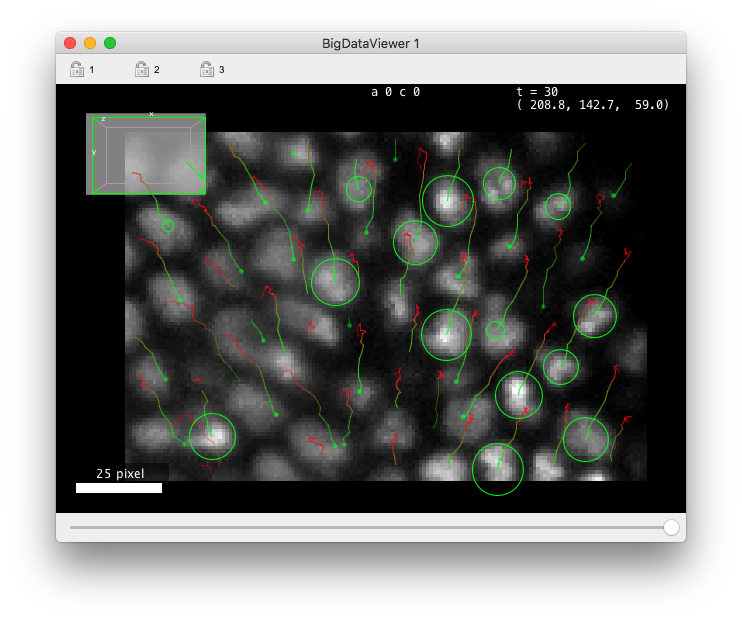
\includegraphics[width=0.6\textwidth,trim=0.5cm .5cm .5cm .5cm,clip]{figures/Mastodon_LinkingResults.png}
     \caption{How tracking results are displayed in BDV views.}
     \label{fig:Tracking results}
\end{figure}  
 
\subsection{Wrapping up.} 

This concludes our first tutorial on automated tracking with Mastodon.
To continue with the next chapter, save the project with the tracks you just generated.

As you can see, after creating a project from a BDV file, the process consists mainly in running in succession the two wizards, one for detection, one for particle linking. 
Even if they provide fully automated tracking, Mastodon is made for interacting with the data as you generate it. 
We will see in a next section how to manually edit a spot, a link or a track even at the finest granularity.
But keep in mind that the tools we quickly surveyed can be used interactively too. 
First the wizards let you go back to change a tracking parameter and check how the results are improved or not. 
Second, because you can specify a region-of-interest (ROI) in the detection step, and select the spots you want to track in the linking step, several runs of these wizard can be combined on different parts of the same image, to accommodate \textit{e.g.} for changing image quality over time, or cell shape over time. 
Mastodon aims at being the workbench for tracking that will get you to results, accommodating a wide range of use cases.


\newpage
\part{Tutorials.}

% Automated tracking.
\newpage
\section{Getting started with Mastodon. Automated tracking.}
\label{Getting_started}

This tutorial is the starting point for new Mastodon users. 
It will walk you through basic operations in Mastodon, opening a dataset and creating a Mastodon project, automatically detect cells and link them, and show you how to use the main views of Mastodon.
We don't go into details, and will revisit the features we survey here later.

\subsection{The image data.}

\subsubsection{Exporting your image to \Bdv file format.}

Mastodon uses \wikilink{BigDataViewer}{\Bdv} (BDV) files as input images.
You need to prepare your images so that they can be opened in the \bdv.

BDV files are used more and more by several software projects in the Fiji ecosystem and beyond. 
This tutorial focuses on Mastodon not on BDV, however we will take a very small detour to explain what makes it fit and how to turn your images into this format. 
If you know already, you can skip this part, because we simply recapitulate what is being explained in the original \Bdv publication~\cite{bdv}.

For this tutorial we will use a ready-made dataset, in the adequate format, but it is a good idea to know how to export or create an image in such a format.
We lazily rely on the excellent \bdv documentation and point directly to the \bdv instructions to prepare your images, \eg depending on whether
\begin{itemize}
	\item they are \wikilink{BigDataViewer\#Exporting_from_ImageJ_Stacks}{opened as an ImageJ stack}, or
	\item they come from a \wikilink{BigDataViewer\#Integration_with_Fiji.27s_SPIMage_Processing_Tools}{SPIM processing pipeline}, or
	\item they come from the \wikilink{BigStitcher}{BigStitcher} plugin~\cite{BigStitcher}, \etc.
\end{itemize}

Once you have prepared your images for opening in the \bdv, you should have a \texttt{.xml} file and a possibly very large \texttt{.h5} file on your computer. The \texttt{.xml} file must be the output of the \bdv data preparation. It should start with the following lines:
\begin{minted}{xml}
<?xml version="1.0" encoding="UTF-8"?>
<SpimData version="0.2">
  <BasePath type="relative">.</BasePath>
  <SequenceDescription>
    <ImageLoader format="bdv.hdf5">
      <hdf5 type="relative">datasethdf5.h5</hdf5>
...
\end{minted}


\subsubsection{Key advantages of the \Bdv file format.}
\label{BDV_advantages}

The BDV file format solves mainly two challenges in image visualization and analysis, that arise with modern microscopy, namely:
\begin{itemize}
    
    \item Modern microscopes can generate images that are very large in size. Much larger that what can be fitted in RAM, even with the increase in computer power. It is now common to find single movies acquired on SPIM microscopes that are several TBs in size. Computers with several TBs of RAM are not so common.
    
    \item Multiple views of the same sample can be acquired, and they need to be visualized in the same viewer. The first use case is also the multi-view images generated by SPIM microscopes, but we can also think of correlative light-electron microscopy.
    
\end{itemize}

If we focus on the first challenge, you see that we need to stream the image data directly from the disk, instead of fully loading it into RAM. 
But at the same time, we need a tool that allows for interactive browsing of the data. 
The view must be responsive to the user input, and not block when it has to load the data from the file. 
The BDV file format offers a clever file format design that does this, coupled to a specialized viewer.
The image data are stored in small chunks corresponding to a neighborhood. As the viewer shows a slice through the image, the required chunks are loaded on demand and cached.
All the chunks are organized in a HDF5 file, which is like a file-system in a file\footnote{\href{https://en.wikipedia.org/wiki/Hierarchical_Data_Format}{\coloredlink{Hierarchical Data Format} on Wikipedia.}}, and accessing single chunks is fast with current computer hardware.
On top of this, the image is also stored as a multi-scale pyramid\footnote{\href{https://en.wikipedia.org/wiki/Pyramid_(image_processing)}{\coloredlink{Multi-scale pyramid} on Wikipedia.}}, to speed-up zooming and unzooming (Figure~\ref{fig:BDVchunks}).
The BDV display component exploits this file format in a clever way, and ensures that the view still answers to user interactions (mouse pan, zoom, clicks \etc) even if the chunks are not full loaded.

\begin{figure}
    \centering
    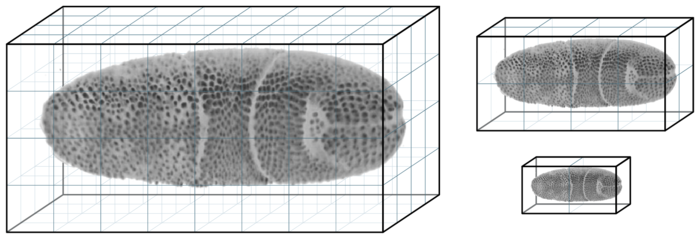
\includegraphics[width=0.6\textwidth]{figures/BdvTikz-pyramidblocks.png}
    \caption{Illustration of the BDV file format storage strategy. The image is stored over several resolution levels (multi-scale pyramid) and in chunks.}
    \label{fig:BDVchunks}
\end{figure}

There are several implementations of this strategy, for instance in Imaris\footnote{\href{http://open.bitplane.com/Default.aspx?tabid=268}{\coloredlink{IMARIS 5.5 File Format Description (IMS).}}} and with the new file format N5\footnote{\href{https://github.com/saalfeldlab/n5}{\coloredlink{N5 API on GitHub.}}} proposed by the Saalfeld lab.
Some of them are inter-compatible.
We will pick the BDV file format all along this document. 
The \Bdv has proved its value and impact on our field.
For instance our previous work on cell lineaging in large images, \wikilink{MaMuT}{MaMuT}, is based on BDV~\cite{MaMuT}.



\subsubsection{The tutorial dataset.}

Mastodon was created specially because we needed to harness very big, multi-view images. We wanted to generate  comprehensive lineages and follow a large number of cells over a very long time.
This accumulation of inflated words is tied to the very large  - in objective disk space  occupation - images we deal with using modern microscopy tools. 
Such datasets might not be optimal for a first contact with Mastodon.
So just for this tutorial we will use a smaller dataset.
It is a small region cut into a movie following the development of a drosophila embryo, acquired by William Lemon in Patrick Keller lab (HHMI, Janelia Farm).
This was created from the example dataset released with the TGMM software~\cite{TGMMpaper}.
You can find it on Zenodo\footnote{\href{https://zenodo.org/record/3336346}{\coloredlink{https://zenodo.org/record/3336346}}} there: \href{https://doi.org/10.5281/zenodo.3336346}{
\includegraphics[height=1.5\fontcharht\font`\B]{figures/zenodo3336346.png}}

It is a zip file that contains 3 files:
\begin{minted}{text}
    14M  datasethdf5.h5
   2.7K  datasethdf5.settings.xml
   8.7K  datasethdf5.xml
\end{minted}

The \texttt{.h5} file is the HDF5 file mentioned above, that contains the image data itself.
The \texttt{data\-sethdf5.xml} is a text file following the XML convention, specific to the BDV file format, that contains information about the the image data and metadata. 
When we want to open a BDV file, we point the reader to this file.
The \texttt{datasethdf5.settings.xml} is an optional file that stores user display parameters, such as channel colors, min and max display value, as well as bookmarks in the data. 
We refer you to the \wikilink{BigDataViewer\#Loading_and_Saving_Settings}{BDV documentation} about this file.
Mastodon uses this settings file to store that same information.

If you open this data in the \Bdv (in Fiji in the \menu{Plugins > BigDataViewer > Open XML/HDF5} menu), you should see something like in figure~\ref{fig:OpeningImage}. 
There is about 70 cells in each of the 30 time-points, arranged in a layer at the top of the sample. 
The deeper part of the sample (low Z coordinates) has some hazy, diffuse signal from which we cannot individualize cells.
As time progresses, the cells move towards the middle part and bottom (high Y coordinates) part of the image, and some of them move deeper in Z, initiating gastrulation.

The goal of this short tutorial is to track all these cells in Mastodon.

\begin{figure}
     \centering
         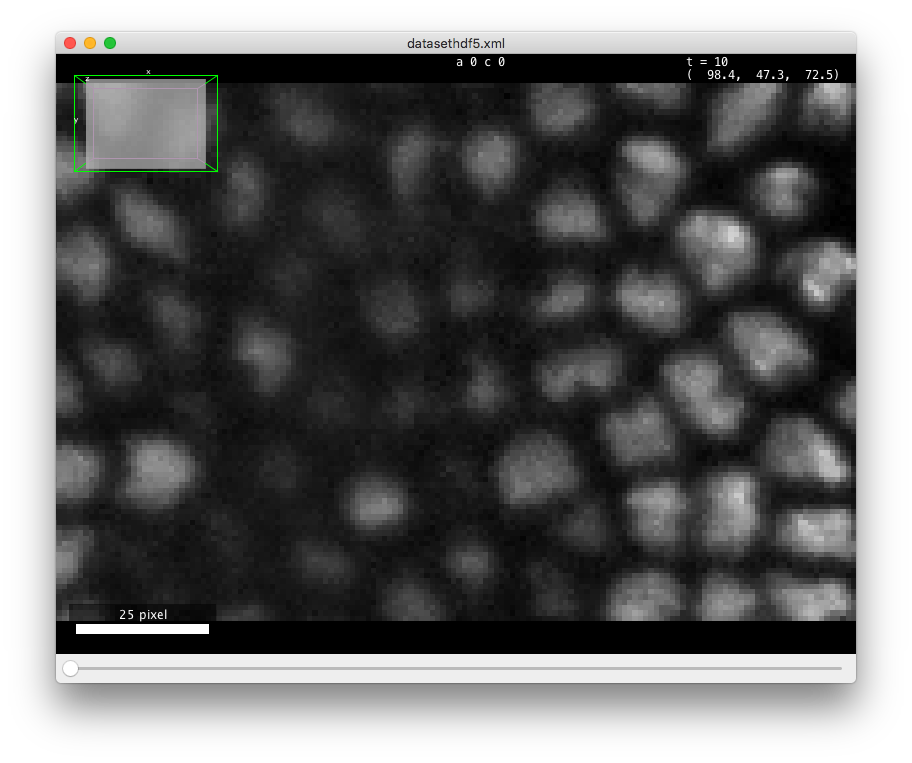
\includegraphics[width=0.3\textwidth]{figures/BDV-imageXY.png}
         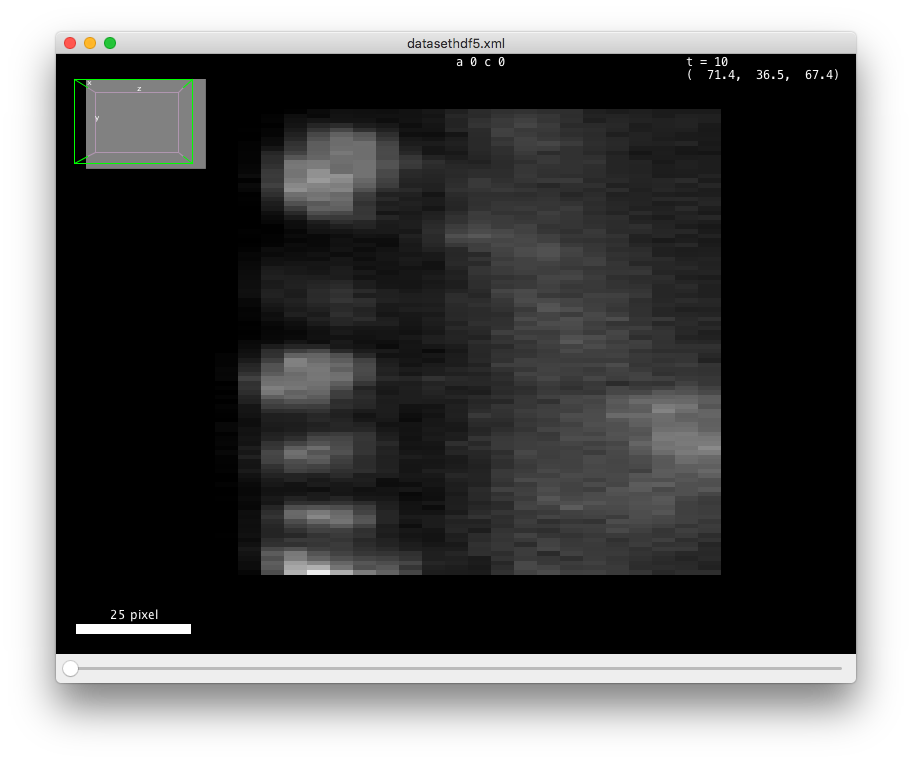
\includegraphics[width=0.3\textwidth]{figures/BDV-imageXZ.png}
         \caption{The tutorial dataset opened in \Bdv, seen along XY (left) and XZ (right)}
     \label{fig:OpeningImage}
\end{figure}  




\subsection{Getting Mastodon.}

As of today, Mastodon is available as a preview. We are still working on adding and validating features.
Nonetheless the preview has everything we need to track these cells.
Also, Mastodon is independent of ImageJ or Fiji, it can operate as a standalone software. 
However we currently distribute it via Fiji, because the updater and the dependency management are so convenient. 
So the first thing to do is to grab Fiji\footnote{\href{http://fiji.sc/}{\coloredlink{http://fiji.sc/}}}, if you do not have it already.

Then launch the \wikilink{Updater}{Fiji updater} and once your Fiji is up to date, click on the \texttt{Manage update site} button.
We will add the \wikilink{Following_an_update_site}{add the Mastodon update site}.
You should find the Mastodon preview site in the list. 
Select it, update Fiji and restart it. 
After restarting, you should find the command \menu{Plugins > Mastodon (preview)} at the bottom of the menu.

\begin{center}
    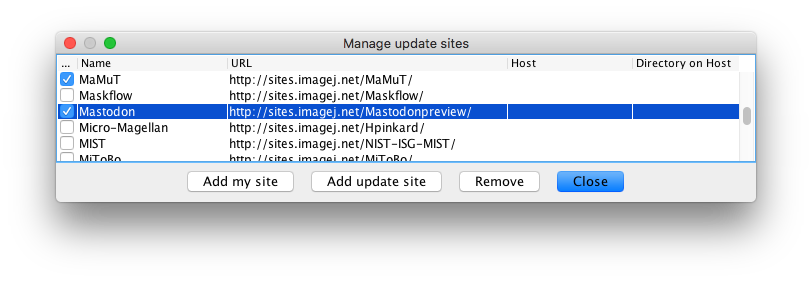
\includegraphics[width=0.7\textwidth]{figures/Mastodon_UpdateSite.png}
\end{center}

\subsection{Creating a new Mastodon project.}

After launching the command, this plain, sober window appears.
\begin{figure}[!htbp]
    \centering
    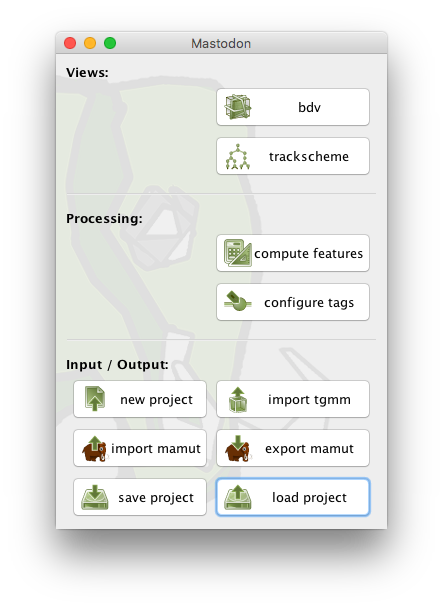
\includegraphics[width=0.3\textwidth]{figures/Mastodon_MainWindow.png}
    \caption{The main window of Mastodon.}
    \label{fig:MastodonMainWindow}
\end{figure}

Click on \menu{new project}, and browse to the \texttt{datasethdf5.xml} file of the XML/HDF5 file pair of the tutorial dataset.
All the buttons that were grayed out should be now enabled. 
Click on the \menu{bdv} button.
A BDV window should appear and if it does everything is right.
\begin{center}
         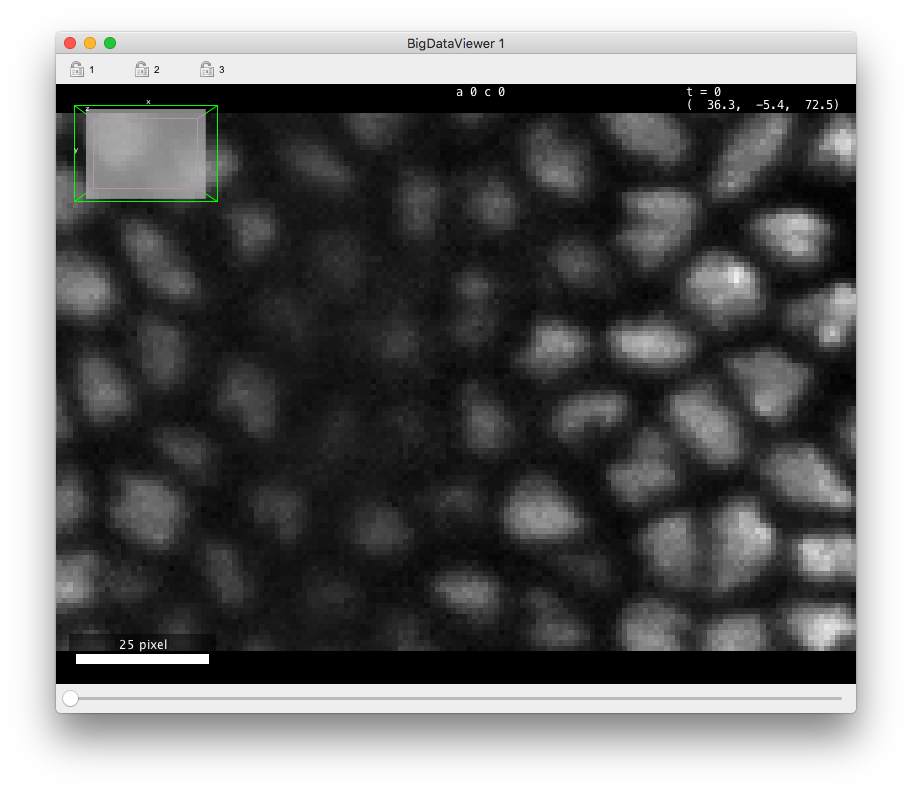
\includegraphics[width=0.4\textwidth]{figures/Mastodon_BDV.png}
\end{center}

It is almost a regular BDV window and if you already know who to use it and the key bindings you should find your marks quickly.
The BDV view displays a \textit{slice} of the image through arbitrary orientation. 
Below we give the commands and key-bindings for navigation in a Mastodon-BDV window. 
They are indeed close to what is found in the standard \Bdv but some changes. 
\textbf{Please note:} You can reconfigure almost everything in Mastodon, as we will see later, including key-bindings.
In this tutorial and the next ones, the key-bindings we present are for the \texttt{Default} configuration.
In the table~\ref{tab:MastodonBDVNavigationKeys} page~\pageref{tab:MastodonBDVNavigationKeys} you will find the key bindings to navigate through the image data.

\begin{table}[!htbp]
    \centering
    
    \caption{Default navigation key-bindings for Mastodon-BDV views.}

    \begin{tabulary}{\textwidth}{L|J}
    
    \toprule
    \textbf{Action}                 & \textbf{Key}              
    \\ \midrule
    
    \multicolumn{2}{c}{\textit{View.}}
    \\ \midrule
    
    Move in X \& Y.                 & \keys{Right-click} and \keys{Drag}
    \\ \midrule
    
    Move in Z.                      & \keys{Mouse-wheel}. Press and hold \keys{\shift} to move faster, \keys{\ctrl} to move slower.
    \\ \midrule
    
    Align view with X / Y / Z axes. &  
    \begin{minipage}[t]{0.7\textwidth}
    \begin{itemize}
        \item  Align with XY plane: \keys{\shift+Z}
        \item Align with YZ plane: \keys{\shift+X}
        \item Align with XZ plane: \keys{\shift+C} or \keys{\shift+Y} 
    \end{itemize}
    The view will rotate around the location you clicked.
    \end{minipage}
    
    \\ \midrule
    
    Zoom / Unzoom.                  & \keys{\ctrl+\shift+Mouse-wheel} or \keys{\cmd+Mouse-wheel}. The view will zoom and unzoom around the mouse location.
    \\ \midrule

    \multicolumn{2}{c}{\textit{Time-points.}}
    \\ \midrule
    
    Next time-point.                & \keys{]} or \keys{M}
    \\ \midrule
    
    Previous time-point.            & \keys{[} or \keys{N}                                                                                     
    \\ \midrule

    \multicolumn{2}{c}{\textit{Bookmarks.}}
    \\ \midrule

    Store a bookmark.               & \keys{\shift+B} then press any key to store a bookmark with this key as name. A bookmark stores the position, zoom and orientation in the view but not the time-point. Bookmarks are saved in display settings file.
    \\ \midrule
    
    Recall a bookmark.              & Press \keys{B} then the key of the bookmark.
    \\ \midrule  
    
    Recall a bookmark orientation.  & Press \keys{O} then the key of the bookmark. Only the orientation of the bookmark will be restored.
    \\ \midrule
    
    \multicolumn{2}{c}{\textit{Image display.}}
    \\ \midrule
    
    Select source 1, 2 \ldots         & Press \keys{1} / \keys{2} \ldots
    \\ \midrule
    
    Brightness and color dialog.    & Press \keys{S}. In this dialog you can adjust the min \& max for each source, select to what sources these min \& max apply and pick a color for each source.
    \\ \midrule
    
    Toggle fused mode.              & Press \keys{F}. In fused mode, several sources are overlaid. Press \keys{\shift+1} / \keys{\shift+2} \ldots to add / remove the source to the view. In single-source mode, only one source is shown.
    \\ \midrule
    
    Visibility and grouping dialog.     & Press \keys{F6}. In this dialog you can define what sources are visible in fused mode, and define groups of sources for use in the grouping mode.
    \\ \midrule
    
    Save / load display settings.       & \keys{F11} / \keys{F12}. This will create a \texttt{XYZ\_settings.xml} file in which the display settings will be saved.
    \\ \bottomrule

\end{tabulary}


    \label{tab:MastodonBDVNavigationKeys}
    \vspace{-10pt}

\end{table}

Now you want to save the project. 
Go back to the main window, and click on the \menu{save project} button.
This will create a single file, called for instance \texttt{drosophila\_crop.mastodon} file. 
This file is actually a zip file that contains the tracks and \textit{links} to the image data.
The image data is kept separate from the Mastodon file, which allows for using it with another software, independently. 
So if you want to transfer or move a full Mastodon project, you need to take the \texttt{.mastodon} file and all the \texttt{.xml} and \texttt{.h5} files from the \Bdv dataset.

Next time you want to open this project, just click on the \menu{load project} button and point the file browser to the \texttt{.mastodon} file.
The image data will be loaded along with the lineages.



\subsection{Detecting cells.}
\label{Detecting_Cells}

\begin{figure}
    \centering
     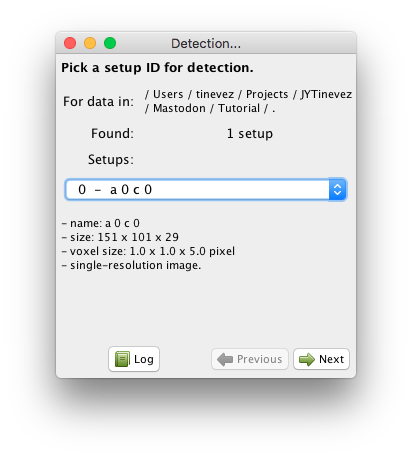
\includegraphics[width=0.4\textwidth]{figures/Mastodon_DetectionWizard_01.png}
     \caption{First panel of the detection wizard.}
     \label{fig:DetectionWizardFirstPanel}
\end{figure}

We want to track automatically all the cells in this dataset, and the first step is therefore to detect them.
Mastodon ships a wizard to perform cell detection. 
It is very much inspired by the \wikilink{TrackMate}{TrackMate} GUI, and if you know this software you will find your marks here.
Also, the algorithms are very close to what was in TrackMate~\cite{TrackMate}, but they have been heavily optimized for Mastodon.

The detection wizard can be launched from the \menu{Plugins > Tracking > Detection...} menu item. 
You should have a window like the one depicted in Figure~\ref{fig:DetectionWizardFirstPanel}.

Like for TrackMate, the automated tracking user interface uses \textit{wizards} to enter parameters, select algorithms, \textit{etc.}
You can navigate back and forth with the \menu{\smallimg{arrow_right.png} Next} and  \menu{\smallimg{arrow_left.png} Previous} buttons. 
The \menu{\smallimg{book.png} Log} button will bring an independent panel where all the activity in the wizard are logged as text. 

This first panel allows for selecting the target \textit{source} on which the detection will be run. 
Since we use the \bdv for images, a channel or a view is stored and displayed as a source. 
A source can have multiple resolutions stored, as explain in paragraph~\ref{BDV_advantages}, but for the data used in this tutorial this is not the case. The sources are nicknamed 'setups' in this panel.
They are numbered from 0 and can be selected from the drop-down list. 
Below the list we try to display the metadata we could retrieve from the \bdv file.
Just pick the first and only channel, and click \menu{\smallimg{arrow_right.png} Next}.

You can now choose to operate only on a rectangular ROI in the image. 
If you check the \textbf{Process only a ROI} button, new controls appear in the panel, and a ROI is drawn into an open BDV view (a new one is created if one is not opened).
The ROI is painted as a wire-frame box, green for vertices that point towards the camera from the displayed slice, and purple for vertices that points away from the camera, below the displayed slice.
The intersection of the ROI box with the displayed slice is painted with a purple semi-transparent overlay, with a white dotted line as borders.
You can control the ROI bounds with the controls in the panel, or by directly dragging the ROI corners in the BDV view.
Time bounds can also be set this way. In our case we want to segment the full image over all time-points, so leave the \textbf{Process only a ROI} button unchecked.

You cannot have non-rectangular ROIs in Mastodon. Nonetheless they are super useful as is. 
You can for instance combine several detection steps using different parameters in different region of your image. Or different time interval.

\begin{center}
     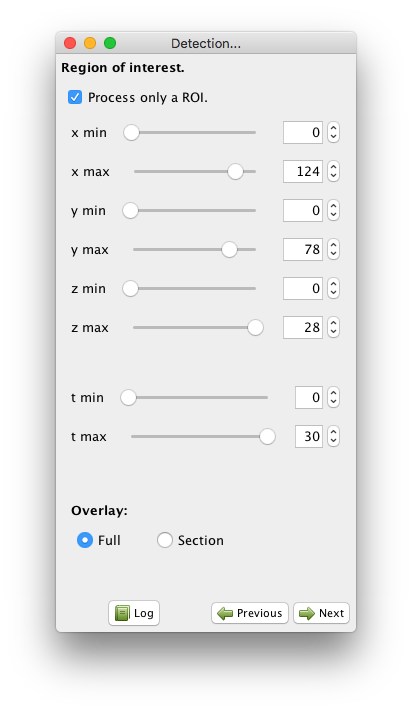
\includegraphics[height=0.25\textheight]{figures/Mastodon_ROIpanel.png}
     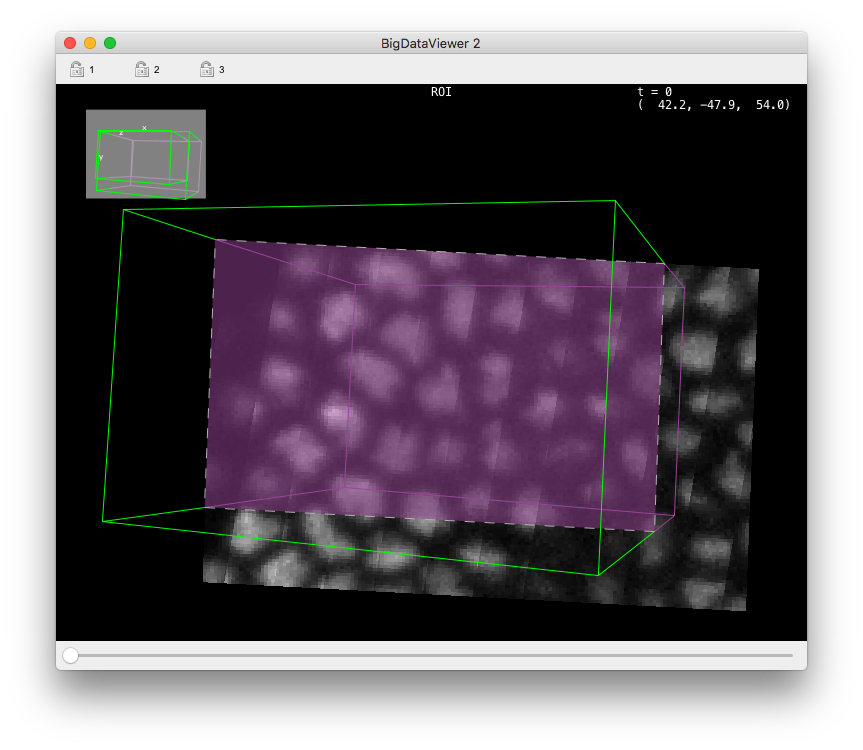
\includegraphics[height=0.25\textheight]{figures/Mastodon_ROIBDV.png}
\end{center}

The next panel lets you choose the detector you want to use.
In vanilla Mastodon, three detectors are available.
Right now, we will use the default one, the \textbf{DoG detector}, which should be good enough for most cases.
DoG means 'difference-of-Gaussians'.
It is an efficient approximation of the LoG ('Laplacian of Gaussian') filter, and there is also a detector in Mastodon based on the latter.

These detectors excel at finding roundish structures in the image that are bright over a dark background.
The structures must have a shape somewhat close to a sphere, but they can accommodate a lot of variability.
As a rule of thumb, if you can define rough estimate of the radius of these structures, they are eligible to be picked up by our detectors. 
This also implies that in Mastodon, we cannot segment complex shapes, or object labeled by their contour (\textit{e.g.} cell membranes), or even exploit these shapes to have an accurate measurements of the volume. 
This is an important limitation of Mastodon.

For now, select the \textbf{DoG detector} and click \menu{\smallimg{arrow_right.png} Next}.
\label{Detection_Cells_DoG_Detector}

Here is briefly  how it works.
The LoG detector, and its approximation the DoG detector, is the best detector for blob-like particles in the presence of noise~\cite{Sage2005}. 
It is based on applying a Laplacian of Gaussian (LoG) filter on the image and looking for local maxima. The result is obtained by summing the second order spatial derivatives of the gaussian- filtered image, and normalizing for scale.
Local maxima in the filtered image yields spot detections. 
Each detected spot is assigned a \textbf{quality} value, that is obtained by taking the intensity value in the LoG filtered image at the location of the spot.
So by properties of the LoG filter, this quality value is larger for :
\begin{itemize}
    \item bright spots;
    \item spots which diameter is close to the specified diameter.
\end{itemize}

The DoG detector requires only two parameters: the estimated diameter of the object we want to detect, and a threshold on the quality value, that will help separating spurious detections from real ones. 
The panel you are presented let you specify these parameters, and preview the resulting detection.
Try with 10 pixels for \textbf{Estimated diameter} and 0 for the \textbf{Quality threshold}.
The click on the \menu{\smallimg{led-icon-eye-green.png} Preview} button.
A preview panel should open shortly, showing detection results on the current frame (Figure~\ref{fig:PreviewDetection}).

\begin{figure}
    \centering
         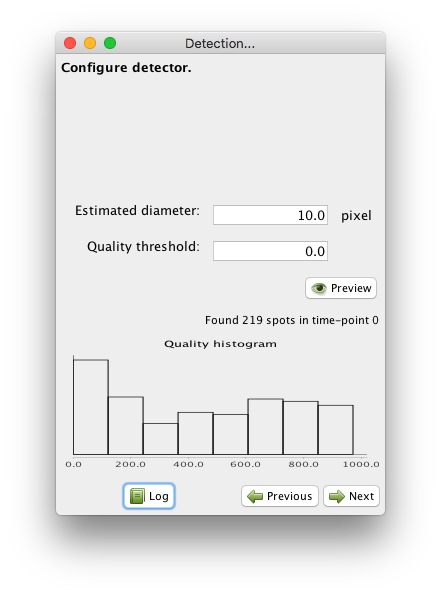
\includegraphics[height=0.25\textheight]{figures/Mastodon_DoGconfig1.png}
         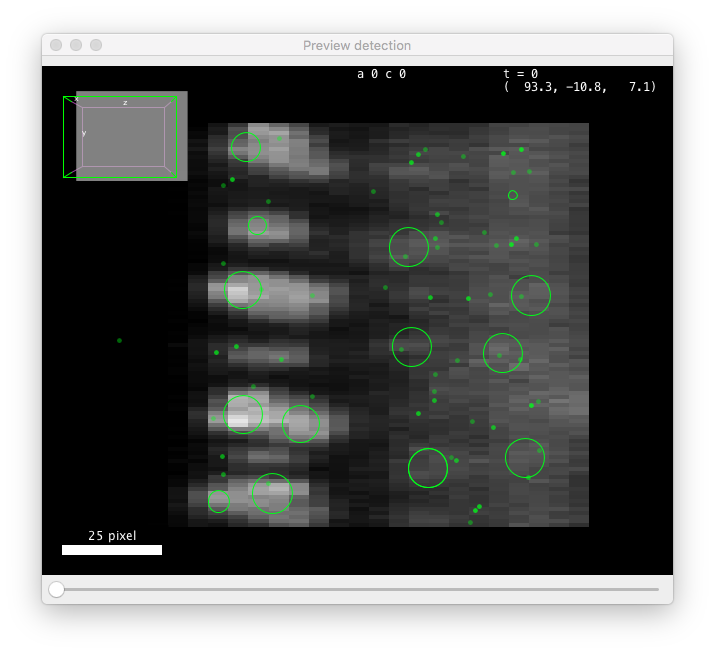
\includegraphics[height=0.25\textheight]{figures/Mastodon_DoGconfig2.png}
    \caption{Previewing detection results.}
    \label{fig:PreviewDetection}
\end{figure}

These values are close but not quite.
You can see that the diameter value is too small to properly grasps the elongated shape of the cells along Z (the BDV view on the left panel above is rotated to show a YZ plane). 
Also the threshold value is too low, and some spurious detections are found below the epithelium.
These spots have a low quality, that manifests as a peak at low value in the quality histogram displayed on the configuration panel.
From the shape of the histogram, we can infer that a threshold value around 100 should work.
However we also need to change the diameter parameter, which will change the range of quality values.
After trial and errors, values around 15 pixels for the diameter and 400 for the threshold seem to work.

Note that you can run the preview on any frame.
You just have to move the time slider on the preview window.
Once you are happy with the parameters, click on the \menu{\smallimg{arrow_right.png} Next} button.
All the frames specified in the ROI (if any) will be processed. 
In our case detection should conclude quickly and the following panel should appear:

We now have more than 1000 cells detected and this concludes the detection step (Figure~\ref{fig:DetectionResults}).
Click on the \menu{\smallimg{accept-icon.png} Finish} button, and the wizard will disappear.

\begin{figure}
    \centering
    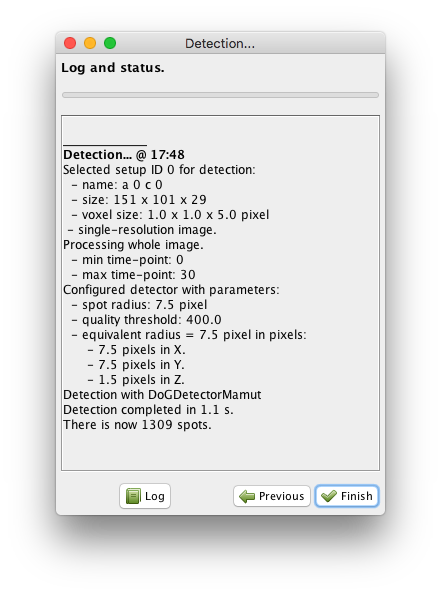
\includegraphics[height=0.40\textwidth, trim=0.5cm 0.5cm .5cm .5cm, clip]{figures/Mastodon_DetectionResuts.png}
    \caption{Detection results.}
    \label{fig:DetectionResults}
\end{figure}

If you have complex images mixing several size of objects, or detection parameters that work for one part of the movie but not for another one, you could restart a new detection now, selecting for instance other parts of the movie with the ROI.
You can do this and more, but for this kind of approach, the \textbf{Advanced DoG detector} offers more configuration capabilities, that will review later.



\subsection{Linking cells.}

What we just did is the detection step. 
It yields one Mastodon spot per cell, but the notion of cell identity propagated over time is missing yet.
The particle linking step just does that.
A particle linking or tracking algorithm accepts a collection of spots, ordered by frames (time-points), and tries to link each spot to the next spot(s) in the next frame or so. 
All the spots you can reach by starting from one spot and navigating across links build a \textit{track}, and in our case it represents one cell (or any other object) followed over time. 
In most cases there is one spot per frame for a track, meaning that that a spot has at most one incoming link (spot from previous frame) and one outgoing kink (spot in next frame). 
But some algorithms can accommodate \textit{e.g.} dividing cells (2 outgoing links for the mother cell going to the two daughter cells) and merging events. There is a vast literature behind tracking algorithms, and it is an active domain of Research. A relatively recent paper compare implementation and list some pros and pitfalls of many of them~\cite{Chenouard2014}.

\subsubsection{Selecting target spots for linking.}

\begin{figure}
    \centering
    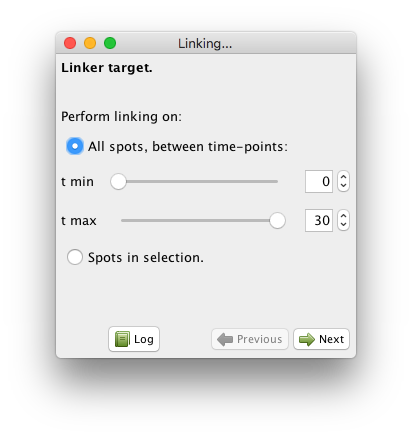
\includegraphics[height=0.3\textwidth,trim=0.5cm .5cm .5cm .5cm,clip]{figures/Mastodon_LinkingWizard_01.png}
    \caption{The first panel of the linking wizard.}
    \label{fig:LinkingWizardFirstPanel}
\end{figure}

Like for the detection step, linking in Mastodon happens in a wizard.
And also like for detection, the linking algorithms currently available in Mastodon are adapted from TrackMate. 
Launch the wizard from the GUI, with the \menu{Plugins > Tracking > Linking...} menu item. 
The first panel you are shown lets you select what spots to include in linking (Figure~\ref{fig:LinkingWizardFirstPanel}). 
There are two modes:
\begin{itemize}
    \item Either you take all the spots between a start and and end frame. By default, all frames are selected.
    \item Either you specify you want to link only the spots that are in the selection. 
    This mode offers a lot of flexibility when facing complicated cases. 
    It is best use along with the selection creator, that we will introduce later in this manual.
\end{itemize}
For now, just leave the parameters as they are, which will include all spots in the linking process, and click next.
You can now choose between several linking algorithms. 

\subsubsection{Available linking algorithms in Mastodon.}

In Mastodon, they fall mainly in two categories.

The first two LAP trackers are based on the \textbf{Linear Assignment Problem (LAP) framework}, first developed by Jaqaman \textit{et al.}~\cite{Jaqaman2008}, with important differences from the original paper described elsewhere~\cite{TrackMate}. 
We focused on this method for it gives us a lot of flexibility and it can be configured easily to handle many cases. 
You can tune it to allow splitting events, where a track splits in two, for instance following a cell that encounters mitosis. 
Merging events are handled too in the same way. More importantly are gap-closing events, where a spot disappear for one frame (because it moves out of focus, because detection failed, ...) but the track manages to recuperates and connect with reappearing spots later.

In Mastodon the LAP algorithms exists in two flavors: a simple one and a not simple one. There are again the same, but the simple ones propose fewer configuration options and a thus more concise configuration panel. In short:
\begin{itemize}
    \item The simple one only allows to deal with gap-closing events, and prevent splitting and merging events to be detected. Also, the costs to link two spots are computed solely based on their respective distance.
    
    \item The not simple one allows to detect any kind of event, so if you need to build tracks that are splitting or merging, you must go for this one. If you want to forbid the detection of gap-closing events, you want to use it as well. Also, you can alter the cost calculation to disfavor the linking of spots that have very different feature values.
\end{itemize}

The third tracker is called \textbf{Linear motion Kalman linker}.
It can deal specifically with linear motion, or particles moving with a roughly constant velocity.
This velocity does not need to be the same for all particles. 
It relies on the Kalman filter\footnote{\href{https://en.wikipedia.org/wiki/Kalman_filter}{\coloredlink{Kalman filter on Wikipedia.}}} to predict the most probable position of a particle undergoing (quasi) constant velocity movement.

\subsubsection{How to pick the right linking algorithm?}

The right choice of a particle linking algorithm is conditioned by the expected motion of the object you track.
As a rule of thumb, you can make a decision following these simple rules:
\begin{itemize}
    
    \item If the objects you track are transported by an active process and have a motion for which the velocity vector changes slowly, then pick the  \textbf{Linear motion Kalman linker}.
    
    \item If the object motion is random (like in Brownian motion) or unknown, pick on the LAP linker. If the objects you track do not divide, nor merge, pick the \textbf{Simple LAP linker}.
    
    \item If the objects divide or merge, or if you want to specify linking costs based on numerical features (like spot mean intensity), then pick the \textbf{LAP linker}.
    
\end{itemize}
In our case, we need the \textbf{Simple LAP linker}. Select it and click \menu{\smallimg{arrow_right.png} Next}.

\subsubsection{Running the Simple LAP linker.}

This linker only requires the specification of three parameters.

The first one is the \textbf{Max linking distance} during frame-to-frame linking. 
It is the distance beyond which linking a spot to another one in the next frame will be forbidden. 
For instance, if you know that your objects move by at most 5~{\textmu}m from one frame to the next, pick a value slightly larger, for instance 6~{\textmu}m.
Distances are expressed in whatever physical units the BDV dataset specified.
In our case it is pixels. 

\begin{center}
    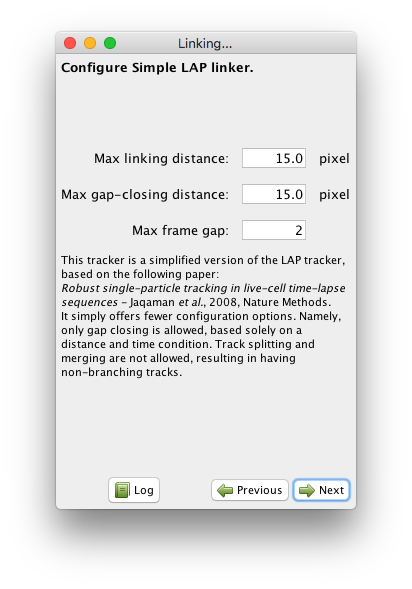
\includegraphics[height=0.25\textheight,trim=0.5cm .5cm .5cm .5cm,clip]{figures/Mastodon_LinkingWizard_03.png}
\end{center}

In practical cases, it can happen that the detection step might miss an object in some frames, then detect again later.
These gaps will result in generating several small tracks for a single objects, which is one of the main course of spurious results when analyzing tracks. 
The simple LAP linker can bridge over missed detections.
It does so by inspecting small tracks that results from frame-to-frame linking, and tries to connect the end of one with the beginning of another one.
The last two parameters of the linker specifies how they are bridged. 
The \textbf{Max gap-closing distance} specifies how far can we look for candidates when we try to bridge the end of a track with the beginning of another one.
The \textbf{Max frame gap} specifies how far they can be in time. 
For instance a Max-frame-gap of 2 means that we can bridge the end of a track at frame $t$ with the beginning of a track at frame $t+2$.
Which results of bridging over detections missed by no more than 1 frame.

In our case, the default parameters turn to work fine. 
Click \menu{\smallimg{arrow_right.png} Next} and the linking will proceed. 
Click on the \menu{\smallimg{accept-icon.png} Finish} button to end the tracking process.
If you have a BDV window opened, it should be updated with the tracking results, like in figure~\ref{fig:Tracking results}.
By default the tracks are represented by colored lines, extending backward in time.
Points in tracks that are close to the current time-point are green and fade to ref for points that are far back in time.
When you change the Z focus, the spots are painted as circle of radius corresponding the the intersection of the sphere with the current Z-plane. 
When the spot sphere does not interest with current Z-plane, it is painted as a small dots.
The points of the track away in time that are not close to the current Z-slice are faded away.
We will see later how to customize the display of tracks. 
 
 
\begin{figure}
    \centering
    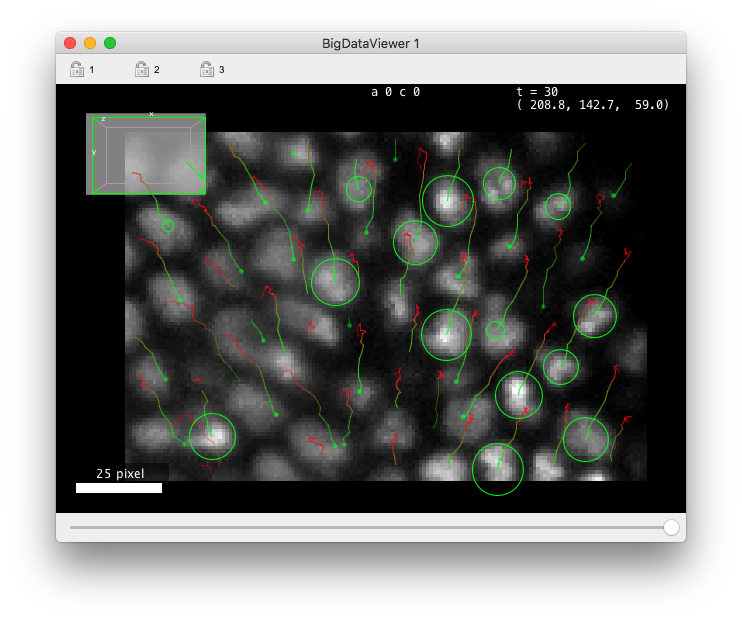
\includegraphics[width=0.6\textwidth,trim=0.5cm .5cm .5cm .5cm,clip]{figures/Mastodon_LinkingResults.png}
     \caption{How tracking results are displayed in BDV views.}
     \label{fig:Tracking results}
\end{figure}  
 
\subsection{Wrapping up.} 

This concludes our first tutorial on automated tracking with Mastodon.
To continue with the next chapter, save the project with the tracks you just generated.

As you can see, after creating a project from a BDV file, the process consists mainly in running in succession the two wizards, one for detection, one for particle linking. 
Even if they provide fully automated tracking, Mastodon is made for interacting with the data as you generate it. 
We will see in a next section how to manually edit a spot, a link or a track even at the finest granularity.
But keep in mind that the tools we quickly surveyed can be used interactively too. 
First the wizards let you go back to change a tracking parameter and check how the results are improved or not. 
Second, because you can specify a region-of-interest (ROI) in the detection step, and select the spots you want to track in the linking step, several runs of these wizard can be combined on different parts of the same image, to accommodate \textit{e.g.} for changing image quality over time, or cell shape over time. 
Mastodon aims at being the workbench for tracking that will get you to results, accommodating a wide range of use cases.


% Manual tracking. TrackScheme.
\newpage
\section{Getting your bearings in large datasets.}

In the previous chapter we have seen how to edit single spots and links in Mastodon, what can be called point-wise editing.
As we said before, the goal of Mastodon is to let you harness very large images, for which the number of annotations can be very large too.
It can be very easy to get lost within such large images and loose track of where we are within the sample image and what cell we follow. 
So we have added several features that are made especially to get your bearings in large datasets.
More than anything, these features are about giving visual cues that ease orientation, and exploit events and signal that would help a human brain get a sense of orientation. 
We took some inspiration from video-games, that are very good at communicating condensed and synthetic information to the player
(but only for a limited part; there is no screenshake when you delete a spot).


\subsection{Bookmarks in the BDV views.}

The \bdv~\cite{bdv} is the image component of Mastodon and is meant to deal with very large images.
It offers interactive and responsive user interaction, and to achieve this without any hardware acceleration, it resorts to only displaying a 2D slice through the data.
This 2D slice can be arbitrarily positioned and oriented. 
When it comes to annotating a 3D image, using a 2D slice is a good approach. 
A full 3D view might actually hinders proper and efficient annotation of the data with a flat 2D screen and a mouse. 
The 3D view leads to ambiguities about the depth positioning of your cursor, and the image data that stands between the camera eye and the plan of interest may hide it.
Parenthetically, these issues with interacting with 3D data are best solved with virtual reality devices, but Mastodon is not a tool that exploit them.
The 2D view offer clarity but conversely does not offer a great feeling of the context. 
We have to live with that.

However to facilitate orienting yourself, or retrieving a key point in the data, you can register bookmarks in the BDV views. 
The bookmarks were already implemented in the \bdv tool itself before its use in Mastodon.
They let you store a position and orientation in space as bookmarks. 
You can later call them again and retrieve said position. 
\begin{itemize}
    \item First move to the position and orientation you want to store in a bookmark.
    \item Then press \keys{\shift+B}. You should see a message prompting you to press another key (Figure~\ref{fig:BDVSettingBookmark}).
    \item Pick one and press it. This key will be used as a tag for this bookmark.
    \item To later retrieve the position and orientation of this bookmark, press \keys{B} then the bookmark's key. The view should animate and restore the stored position and time-point.
    \item \keys{O} does the same things, but only restore the bookmark orientation, not its position.
\end{itemize}

You can have many bookmarks, all identified by the key you press after the bookmark command.
Bookmarks are saved with the BDV settings file that also saves the channel color and display range.
You can save such a file with the \menu{File > Save BDV Settings} or the \keys{F11} key.
The settings file is loaded when a new BDV window is displayed.

\begin{figure}
    \centering
    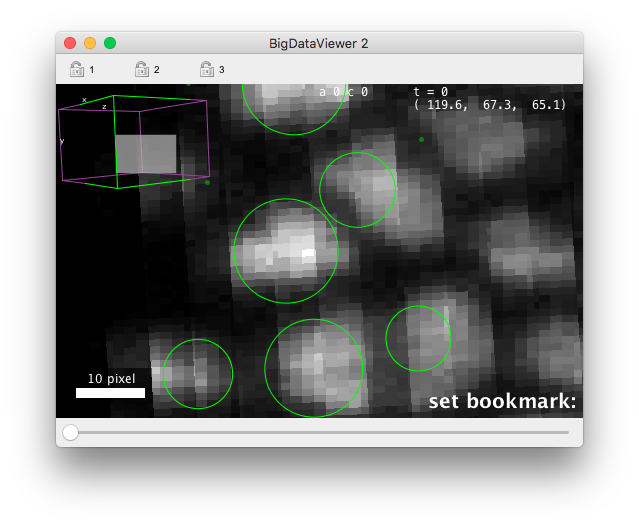
\includegraphics[height=0.27\textheight]{figures/Mastodon_SettingBookmark.png}
    
    \caption{Settings a bookmark in a BDV view.  }
    \label{fig:BDVSettingBookmark}
\end{figure}


\subsection{View modes in BDV.}
\label{sec:BDVViewModes}

TODO TODO TODO



\subsection{Linking several views together.}

You can generate as many views as you want in Mastodon, and you can link several of them via the lock system \smallimg{lock.png}.
This is a good way to improve the perception of context, by linking several views that display for instance a close-up view of the data and another view displaying a bird-eye view of it.
We already presented this feature in the Section~\ref{sec:LinkingViews} page~\pageref{sec:LinkingViews}. 
The figure~\ref{fig:ViewsInSync} page~\pageref{fig:ViewsInSync} shows an example of a view configuration with three views in sync, showing each a different level of desired information.
We direct you there for details on how to use the lock system.


\subsection{In \TrackScheme everything is animated.}

If you went through the previous tutorial, you probably noticed that editing events are associated with animations in \TrackScheme.
For instance, if you delete a link in the middle of a track, the 'bottom' part of the track will move to the left side of TrackScheme, in a quick animation.
If you undo the deletion, the branch will move back to its original place the same way. 
Deleting a spot makes it fade rather than disappear.
These animations are more than a toy.
Something we learned that hard way with MaMuT~\cite{MaMuT} is that point-wise editing the data can completely confuse and disorient the user.
A single link deletion will generate a big rearrangement in the track hierarchy, and therefore will change the \TrackScheme view a lot. 
Without any subtle cues to the user, these changes will disorient them quickly.
Animating the editing events is a great way to hint them about what happens to the data modify in a user-friendly way.

We also added some fluidity and inertia in \TrackScheme navigation. 
In the TrackMate~\cite{TrackMate} and MaMuT~\cite{MaMuT} version of \TrackScheme, panning and zooming were done in discrete discontinuous steps, that would also lead to confusion.
In Mastodon, moving and zooming are done continuously. 
There is even some inertia again to emulate interacting with a tangible panel.



\subsection{Spatial context in TrackScheme.}
\label{sec:SpatialContext}

There are situations where the density of cells displayed in \TrackScheme is so high that even at high zoom level this view is barely useful. 
The hierarchical arrangement of tracks in \TrackScheme is handy to grasp how tracks behave over time.
But since it eliminates spatial information, the neighbors of a track do not bring information to it.

The spatial context in \TrackScheme reconciles spatial information with the hierarchical layout. 
In \TrackScheme views, the toolbar has a \menu{context} list box, from which you can select between \texttt{full graph} and the names of all the BDV views currently opened (typically \texttt{BigDataViewer 1}, \etc).
When \texttt{full graph} is selected, the full lineage data is shown in \TrackScheme. 
This is the classic view.
If you pick an item corresponding to an opened BDV view, then this \TrackScheme view will only display the lineages of the cells currently displayed in the target BDV view. 
And the \TrackScheme view will be updated (and animated) as you pan, move in Z, zoom or unzoom the BDV view (Figure~\ref{fig:SpatialContext}). 

Try it now with the data from the previous tutorial.
Open a BDV view and a \TrackScheme view.
In the \TrackScheme view, select the \texttt{BigDataViewer 1} item (it might not be 1 in your case).
Then in the BDV view, zoom so that almost only one cell is displayed. 
The \TrackScheme view should display considerably fewer tracks. 
As you unzoom, some lineages will appear in \TrackScheme.
You will probably see that some lineages appear in gray, with dashed lines.
They are called "ghost" lineages: 
These are the lineages of cells that are not within the BDV view at the time-point currently displayed, but that will enter this view later or earlier in time. 
The context feature is immensely useful when studying tissue development or coordinated cells movement. 


\begin{figure}
    \null\hfill
    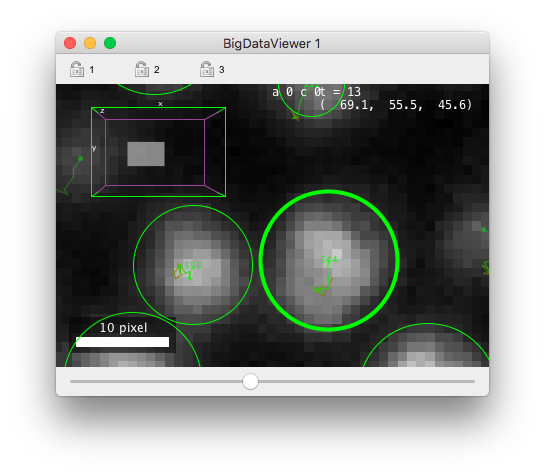
\includegraphics[width=0.32\textwidth]{figures/Mastodon_Context1.png}
    \hfill
    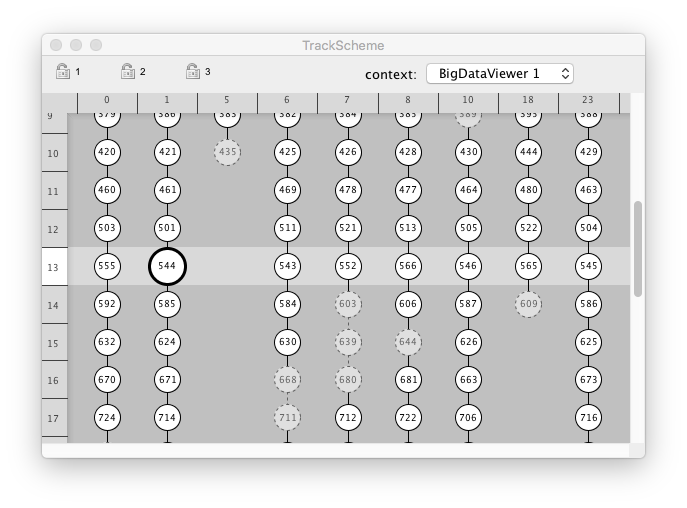
\includegraphics[width=0.38\textwidth]{figures/Mastodon_Context2.png}
    \hfill
    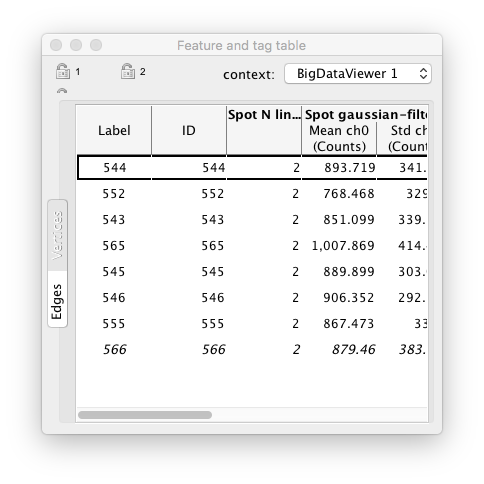
\includegraphics[width=0.25\textwidth]{figures/Mastodon_Context3.png}
    \hfill\null
    
    \caption{Context in Mastodon. The context displayed in \TrackScheme (center) and the table (right, explained in the section~\ref{sec:DataTables} page~\pageref{sec:DataTables}) is determined by what is currently displayed in the BDV window (left). The content displayed in \TrackScheme and the table id updated live as the view in the BDV window is changed by the user. }
    \label{fig:SpatialContext}
\end{figure}

% Orienting in Mastodon.
\newpage
\section{Numerical features and tags. The table view.}

Mastodon is a tracking and lineaging tool.
Its output is a collection of tracks, and the analysis of these tracks to yield statistics on \eg velocity, displacement \etc is carried out in another software package such as MATLAB or Python.
Nonetheless you will find in Mastodon tools to compute \textit{numerical features} on data item. 
Numerical features are numbers that can be calculated on spots, links and tracks of the data. 
For instance there are feature for the number of links that touch a spot, or the displacement of a link or the number of spots in a track.
You can find them within Mastodon because it is convenient, but also because they are very useful for the interactive exploration of your data. 
Coupled with feature-based coloring, the display and sorting of values in the table view and the selection creator tool, they can considerably accelerate and facilitate making sense of the data.

Numerical features are numbers that classically relate to a physical quantity.
When we need to \textit{categorize} items, we rely on \textit{tags}.
We describe them just below. 
This chapter will also show you how to compute numerical features and create a coloring view from the feature values and  tags.
Doing so, we will introduce the third kind of data view in Mastodon: the data tables.


\subsection{Tags and tag-sets.}

As we said above, every-time you need to categorize certain data items, or need to visualize categories, you should rely on tags.
Let's suppose that you are investigating the trajectories of cells in a developing embryo from an early stage to a stage where the embryo is polarized.
Some cells will migrate to the anterior part, some others to the posterior part, \etc. 
You might want to tag cell tracks with the \texttt{Anterior} or \texttt{Posterior} tag, to investigate where do these cell come from in the early embryo.
Or let's say that you are curating the results of the automated tracking on a large images. 
The tracking results might have some inaccuracies, and you want to correct them for important tracks.
Because there is a lot of tracks, you share the workload with some colleagues. 
You work asynchronously with them, editing the Mastodon file one after another. 
Doing so, you can use tags in Mastodon to mark some tracks as reviewed by you.
Your colleagues will use a tag for themselves, to ensure that no two scientists are reviewing the same track twice.
All the cells that are not tagged in this categorisation are still waiting to be reviewed. 

In Mastodon, a categorization corresponds to a \textbf{tag-set}.
A tag-set defines a property that can have a reasonable number of discrete values, or \textbf{tags}.
In the first of the two examples above, \texttt{Location} would be a tag-set to specify the location of cells.
\texttt{Anterior} and \texttt{Posterior} would be two tags belonging to the \texttt{Location} tag-set.
In the second example, \texttt{Reviewed by} would be a tag-set, and \texttt{Mette}, \texttt{Pavel}, \texttt{Tobias} and \texttt{Jean-Yves} would be 4 tags of this tag-set.

You can assign tags to spots and links.
To assign a tag to a whole track, you have to assign this tag to all the spots and links of this track.
One data item (a spot or a ling) can have 1 or 0 tags per existing tag-set.
But they can be categorized by as many tag-sets as there is.
For instance, a spot can have the tag \texttt{Anterior} in the \texttt{Location} tag-set, and the tag \texttt{Pavel} in the \texttt{Reviewed by} tag-set. 
Or it can be not tagged in the \texttt{Reviewed by} tag-set.
But it cannot have both the tag \texttt{Mette} and the tag \texttt{Tobias} because they belong to the same tag-set.
Each tag-set works independently, and clearing a tag-set does not affect the others even for one data item.
Now that we set things straight, let's see how to create tag-sets.
We will base the demonstration in this chapter on the data we generated in the tutorial chapter~\ref{sec:GettingStarted}.


\subsubsection{Creating tag-sets.}

On the main window (see figure~\ref{fig:MastodonMainWindow} page~\pageref{fig:MastodonMainWindow}), there is a button \menu{configure tags}. 
Pressing it opens the tag-set dialog. 
Right now, it appears as an empty table made of two columns (Figure~\ref{fig:CreateTagSet}a). 
This is where you enter tag-sets and tags.

Press the \smallimg{add.png} button on the left column to create a new tag-set. 
A default name is shown for the tag-set, that you can edit.
You can also directly press the  \keys{\return} key to immediately start editing the new tag-set.
Let's say we want to create the location tag we talked about before.
Type \texttt{Location} in the text field. 
An empty line followed by a \smallimg{add.png} button should appear on the right column.
This is where you will enter the tags of this tag-set.
Click on this button, or press the \keys{\tab} key followed by the \keys{\return} key to create a new tag.
For instance, the \texttt{Anterior} tag.
Note that a tag is only made of a label (the text) and a color.
The color will be used in Mastodon views.
Create a second tag for the same tag-set called \texttt{Posterior}.
Pick the color as you like. 
Now try to create another tag-set called \texttt{Reviewed by} and create some tags in this tag-set (Figure~\ref{fig:CreateTagSet}b). 
The tag-set dialog is normally fully navigable with the \keys{\tab}, \keys{\arrowkeyup} and \keys{\arrowkeydown} keys, so that you can enter tags quickly if you have a lot of them.
You can create new tag-set or new tags with the \keys{\return} key, and delete them either with the \keys{\del} key or by pressing the \smallimg{delete.png} button.

When you are finished, press the \menu{OK} button.


\begin{figure}
    \centering
    \null\hfill
    \subfloat[]{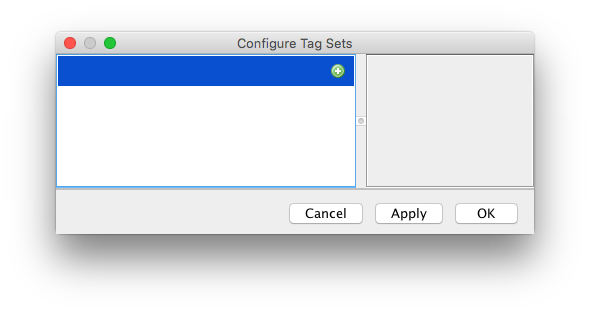
\includegraphics[height=0.15\textheight]{figures/Mastodon_ConfigureTagSet_1.png}}
    \hfill
    \subfloat[]{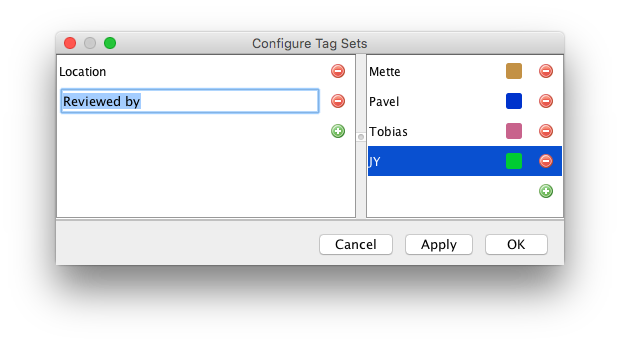
\includegraphics[height=0.15\textheight,trim=0.5cm .5cm .5cm .5cm,clip]{figures/Mastodon_ConfigureTagSet_2.png}}
    \hfill\null
    
    \caption{Creating tag-sets and tags. \textbf{a.}~The empty tag-set dialog. \textbf{b.}~After adding two tag-sets and six tags.  }
    \label{fig:CreateTagSet}
\end{figure}


\subsubsection{Assigning tags to data items.}
\label{sec:AssigningTags}

Tags are set via the selection tool, presented above (chapter~\ref{sec:SelectionTool} page~\pageref{sec:SelectionTool}).
Once you have some spots and links in the selection, you can assign a tag to it via the \menu{Edit > Tags > The tag set name > The tag label} menu.
The menu content will be updated with the tag-sets and tags you defined in the tag-set dialog, described above (Figure~\ref{fig:AssignTagSetMenu}).
This will work in any Mastodon views, BDV or \TrackScheme.

\begin{figure}
    \centering
    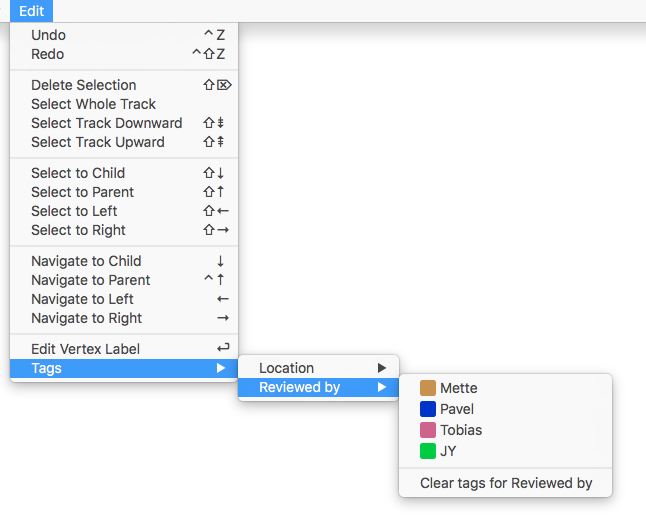
\includegraphics[height=0.2\textheight]{figures/Mastodon_ColorByTagSet_1.png}
    
    \caption{The menu item to assign tag-sets and tags to the current selection. }
    \label{fig:AssignTagSetMenu}
\end{figure}


\TrackScheme ships a second way to set tags quickly from the keyboard.
After selecting the spots and links of interest, press the \keys{Y} key.
A floating menu should appear on the left part of the view panel (Figure~\ref{fig:AssignTagSetShortcut}). 
There is a bit of naming clash in the floating menu.
Here, tag-sets are called \textit{tags} and tags are called \textit{labels}.
Select the desired tag-set with the \keys{1}, \keys{2}, .. keys.
The menu now shows the tags defined within this tag-set, that you can select the same way.
Note that there is a way to remove all the tags over all the tag-sets on the selection by pressing \keys{\shift+\del} on the first menu, or just the tags of the selected tag-set by pressing \keys{0} on the second menu.


\begin{figure}
    \centering
    \null\hfill
    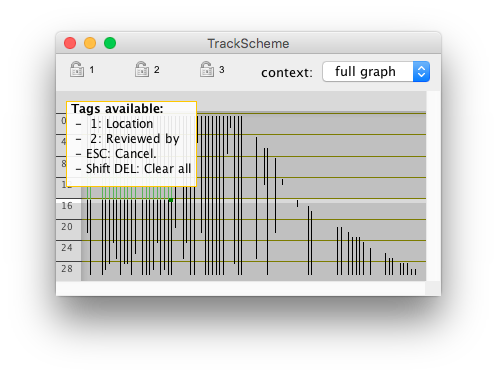
\includegraphics[height=0.2\textheight]{figures/Mastodon_ColorByTagSet_2.png}
    \hfill
    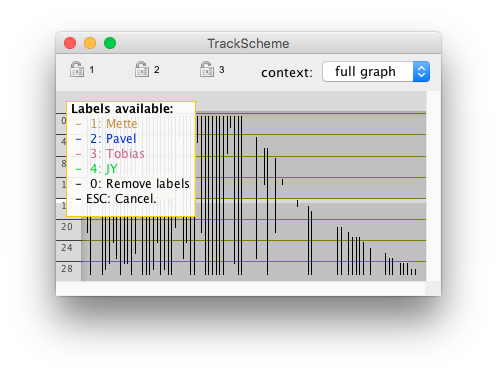
\includegraphics[height=0.2\textheight,trim=0.5cm .5cm .5cm .5cm,clip]{figures/Mastodon_ColorByTagSet_3.png}
    \hfill\null
    
    \caption{Assigning tags in \TrackScheme. After pressing the \menu{Y} key this floating menu is shown, that can be navigated with the digit keys.  }
    \label{fig:AssignTagSetShortcut}
\end{figure}



\subsubsection{Coloring views by tag-sets.}

The tags we just defined and assigned can be used in with the views, to highlight the items that are tagged. 
In the \menu{View > Coloring} menu of any view in Mastodon, you will find a sub-menu updated with the tag-sets you created among other choices (Figure~\ref{fig:ColorByTagSetMenu}). 
By default, newly created views are colored with the \menu{None} coloring mode, which simply colors all the spots and links the same way, taking colors from render settings. 
If you select a mode corresponding to a tag-set, tagged spots and links will appear painted with the color you chose for the tags of this tag-set (Figure~\ref{fig:ColorByTagSetTrackScheme}).
This is very handy to mark some locations in the image or highlight interesting tracks in the data.
Later we will see that tags can be used to retrieve specific items for further processing.
Finally, in \TrackScheme there is an option to show a legend of the current coloring mode.
You can toggle it on or off and set the location of this legend in the \menu{View > Colorbar} menu.

\begin{figure}
    \centering
    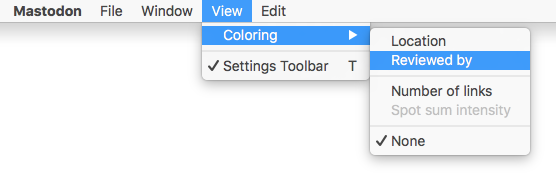
\includegraphics[height=0.1\textheight]{figures/Mastodon_ColorByTagSet_4.png}
    
    \caption{The coloring menu, updated with the tag-sets. }
    \label{fig:ColorByTagSetMenu}
\end{figure}

\begin{figure}
    \centering
    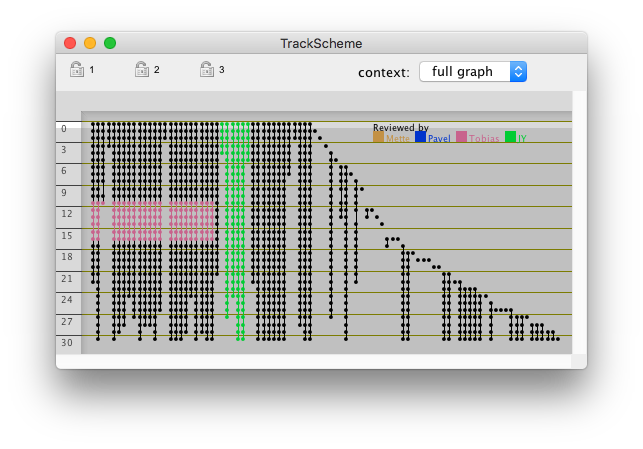
\includegraphics[height=0.25\textheight]{figures/Mastodon_ColorByTagSet_5.png}
    
    \caption{Coloring with tag-sets in \TrackScheme. }
    \label{fig:ColorByTagSetTrackScheme}
\end{figure}


\subsection{Numerical features.}

Numerical features are values that are calculated from the data.
For instance the mean intensity within a spot, or the displacement along a link.
They are very generic: the main restrictions is that there must be a data item (a spot or a link) per feature value. 
But the feature itself can be scalar, non-scalar, real, integer, a string, a vector, 
\etc.
They are \textit{labile}. 
Because they are defined for a data item, they will become invalid as soon as the data item changes.
Think of what happens to the spot mean intensity if the spot is moved over the image for instance.
Because we want to accommodate extensibility and large data, we have to use a special system that we describe below. 

\subsubsection{Feature computation.}

Numerical feature values are calculated by \textbf{feature computers}.
Feature computers are actually specialized Mastodon plugins, made so that it is easy for a 3rd party (you) to implement their own features in Mastodon.
We explain you to write your own feature computer in the second part of this manual, dedicated to technical information.

Because feature computation can take very long on large images, you have to trigger it manually.
On Mastodon main window, you can find a button \texttt{compute features} button.
Pressing it will show the feature computation dialog (Figure~\ref{fig:FeatureComputationDialog}).
The feature computers are listed on the left panel.
Clicking on the computer name displays some information about the feature they compute in the right panel. 
Note that they are named 'features' on this panel, but they are in reality the feature computers.
For instance if you click on the \texttt{Spot gaussian-filtered intensity}, you will see in the information panel that this computer generates a feature for the mean intensity (weighted by a gaussian) and its standard deviation within a spot.
Note also that they can have dependencies.
For instance, the \texttt{Link velocity} feature computer depends on the \texttt{Link displacement} feature to be present at the time of computation.

\begin{figure}
    \centering
    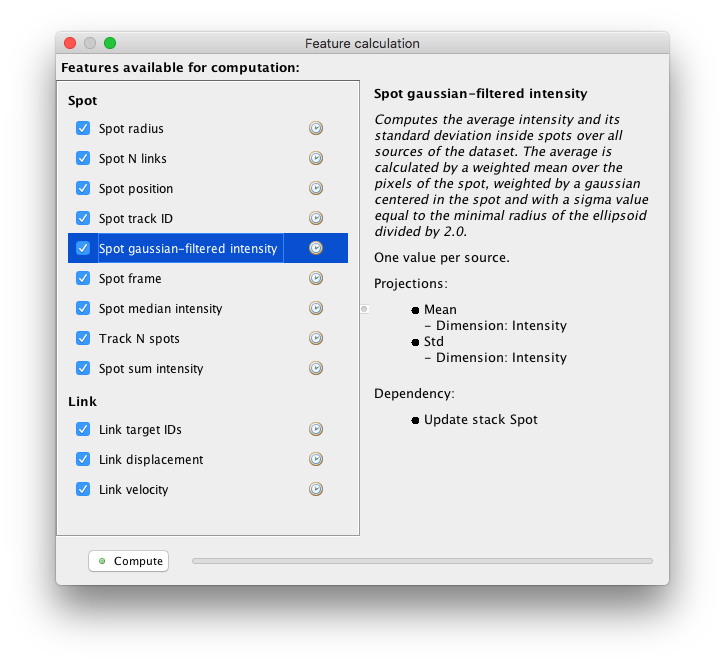
\includegraphics[height=0.3\textheight]{figures/Mastodon_FeatureComputation_1.png}
    
    \caption{The feature computation dialog. }
    \label{fig:FeatureComputationDialog}
\end{figure}

The check-box on the left of each feature computer name triggers whether they will be part of the next feature computation.
Press the \menu{\smallimg{bullet_green.png}Compute} button to trigger computation of features.

Once the computation of all the features is complete, all the small clock icons that were shown right to the feature computer names now turned to a green dot\smallimg{bullet_green.png}.
This is how we keep track of the validity of the feature values.
Since the feature computation is triggered manually, and that a feature value might invalidated if the data changes (new spots added, removed, moved, changed the radius, added or removed some links), this icon serves as a signal for feature value de-synchronization.     
If the icon is shows as a clock~\smallimg{time.png}, it means that the data changed since the last feature computation, and that the feature values are out of sync. 
If is shows a green dot\smallimg{bullet_green.png}, then the data did not change since last computation, and the feature values are sure to be valid. 
This is very important for proper interpretation of the data, and you will have to show the computation dialog often just to check the feature values validity. 
By the way, you can check now how the validity flag works. 
While keeping the feature computation dialog open, move a spot in a BDV view. 
You should see that all the green dot icons now turn to the clock icon.
Also, if you now deselect some feature computers before launching a new computation, the validity flag will not turn to the green dot icon for those feature computers.

You probably have noticed, thanks to the progress bar, that the intensity-related features are the ones that take the most time to compute. 
Indeed, they require loading all of the data blocks on which there are spots.
This could  rapidly become cumbersome for large datasets, if you have to recompute all of the features every-time a spot is added or edited. 
Fortunately we implemented an update mechanism for feature computation.
After the first computation, which possible takes very long, only the spots that have been added or modified since the last computation are visited.
The details of the update mechanism are explained in the technical part of this manual, chapter~\ref{sec:FeatureComputationUpdateMechanism} page~\pageref{sec:FeatureComputationUpdateMechanism}.

Now that we have feature values computed, we would like to inspect them and export them for further analysis.
This is the role of the table view, but before getting to it, we will make a little detour to showing how to use features to generate coloring, accelerating updates of computation and saving them to disk.


\subsubsection{Coloring views by numerical features.}
\label{sec:ConfigureColorModes}

We have seen above that tag-sets could be used to generate coloring of the data items shown in a view. 
Indeed, in the \menu{View > Coloring} menu of each view, that tag-sets are listed and when selected, are used to assign a color to each data item.
We can do something similar with feature values, except that feature based coloring requires more input from us.

Feature color modes need to be created first, and this is done in a dedicated user interface. 
Select the \menu{File > Preferences} menu item in the main window or any view.
The preferences dialog is shown.
It is organized with a side-bar on the left that contains the various items that can be configured in Mastodon. 
Parenthetically, you can see that you can configure the display style of the \TrackScheme and BDV views, and the keymaps. 
But we will see this later.
In the sidebar select \menu{Feature Color Modes}.
The panel on the right now display the feature color mode configuration panel (Figure~\ref{fig:FeatureColorModeConfig1}).

Its top line has a drop-down list that contains all the color modes already defined. 
Right now, there is only one, called \textbf{Number of links}.
As the \textbf{\textit{built-in}} suffix indicates, it is a built-in color modes, and it cannot be edited. 
To create a new one you must duplicate it and rename the new one.   
Do so by clicking on the \menu{Duplicate} button, then on \menu{Rename}.
Let's create a color mode that color spots and links based on the mean intensity inside the spots, that we would call \textbf{Mean intensity}.

\begin{figure}
    \centering
    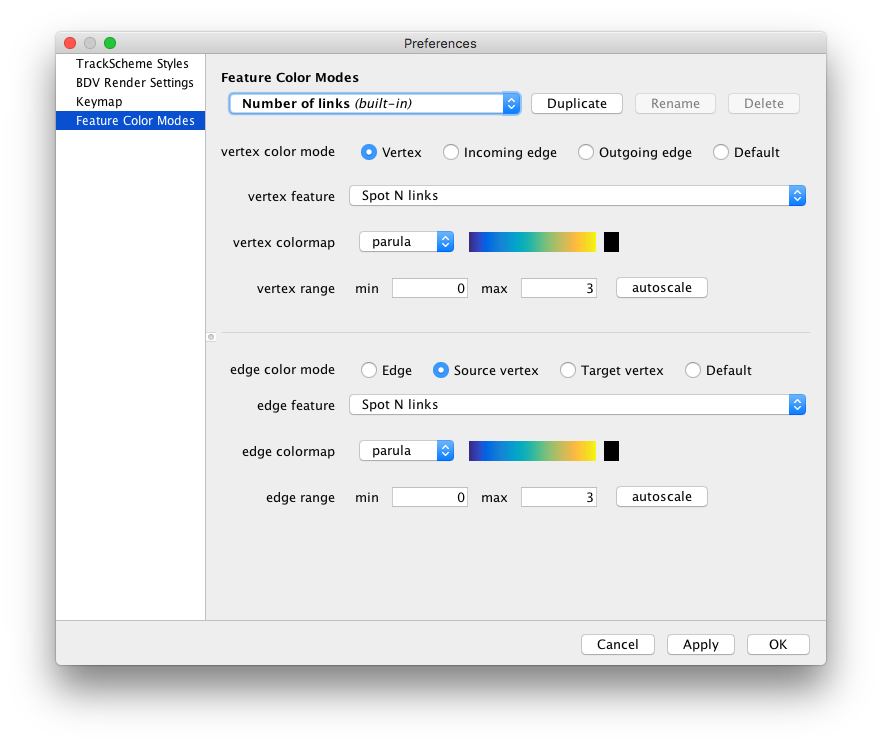
\includegraphics[height=0.3\textheight]{figures/Mastodon_FeatureColorModeConfig_1.png}
    
    \caption{The feature color mode configuration preference dialog. }
    \label{fig:FeatureColorModeConfig1}
\end{figure}

The rest of the configuration panel is made of two parts.
The top part configures the vertex coloring, or how we color spots.
The bottom part configures the edge coloring, or how we color links. 
In Mastodon the data is organized in a mathematical graph\footnote{\href{https://en.wikipedia.org/wiki/Graph_(discrete_mathematics)}{Mathematical graphs on Wikipedia \coloredlink{https://en.wikipedia.org/wiki/Graph\_(discrete\_mathematics)}}}, in which the vertices are the spots, and the edges are the links that connect spots from one frame to another, so you will sometimes find in Mastodon and in this manual the vocables vertex and edge to design a spot and a link respectively. 
The vertex color mode specifies where do we take colors from. 
You can choose between:
\begin{itemize}
    \item \texttt{Vertex}, which means a spot will take its color from a feature value it owns.
    \item \texttt{Incoming edge}, which means a spot will take its color from a feature value owned by the single incoming link that targets this spot. This is the link backward in time. If there are no such links or more than one, then the default color is used.
    \item \texttt{Outgoing edge} is the same thing, but for the link forward in time. 
    \item \texttt{Default} mode does not rely on feature values but simply uses the default color in the view.
\end{itemize}

\noindent Depending on the mode you chose, the content of the drop-down list below, called \texttt{Vertex feature}, will change to reflect either the list of spot features or the link features.
Select \textbf{Vertex} as a color mode and \textbf{Spot gaussian-filtered intensity} as feature.
Two new drop-down list appear on the right of the feature list. 
One contains the list of projections in the feature and the second one contains the list of channels in the dataset. 

We need to explain a bit what are \textbf{feature projections}.
We said above that a feature could be roughly anything numerical, and was not necessarily a scalar. 
It could be a vector, a tensor, a complex number, \etc.
However to be usable and useful in Mastodon, features are required to expose a sensible list of projections that compose them.
Feature projections are scalar and real values that can decompose or project a feature on a real axis.
How they are defined is up to the person that created the feature computer, but we can rely on the \textit{hope} that they choose wisely. 
For instance, a feature that gives the velocity vector of a link will reasonably expose 3 projections, one for each of the X, Y and Z component of the vector. 
Or maybe the polar angle, azimuthal angle and norm of this vector.
Or maybe the 6 projections since they can be calculated on the fly. 
A complex feature value will reasonably expose 2 projections, one for the real part, one of the imaginary part.
\textit{Etc}.
The \texttt{Spot gaussian-filtered intensity} feature has two projections, one for the mean value of the intensity within a spot and the standard deviation of this intensity.
Since both can be computed on any of the channel present in the dataset, their number is multiplied by the number of channels. 
The configuration panel changes according to the number of projections in a feature and its multiplicity (Figure~\ref{fig:FeatureColorModeConfig2}). 
For features that are made of one real value with no multiplicity, the projection list is superfluous and not shown.
In our case, we simply want the mean of the only channel in the dataset.

Coming back to the color mode configuration, next we need to pick a color-map.
A color-map acts as the LUT for an image, and maps a color to a certain value. 
Mastodon ships about 20 of them, many taken from the MatPlotLib project\footnote{\coloredlink{\url{https://matplotlib.org/3.1.1/gallery/color/colormap_reference.html}}}.
Finally, you have to specify a min value and a max value that will act as the brightness and contrast values for an image.
Values below the min you defined will all be displayed with the first color of the color-map and values larger than the max with last.
The black square you see next to the graded representation of the color-map is the color used for data items for which the feature value is not present or undefined (division by zero, \etc).
The \texttt{autoscale} button computes the min and max automatically from the feature currently selected with the values taken from the last feature computation.

The edge coloring works exactly the same, except for the edge color mode.
\begin{itemize}
    \item \texttt{Edge} means that a link will be colored by a feature value it owns.
    \item \texttt{Source vertex} will take a feature value from the source spot of this link, that is, the first in time.
    \item \texttt{Target vertex} does the same but for the last spot in time of this link. 
    \item \texttt{Default} mode does not rely on feature values but simply uses the default color in the view.
\end{itemize}
\noindent To build our example feature color mode, choose \texttt{Source vertex} as color mode, and use for instance the \texttt{viridis} color-map along with 700 and 1100 for min and max values.
Do the same for the vertex color mode (Figure~\ref{fig:FeatureColorModeConfig2}).


\begin{figure}
    \centering
    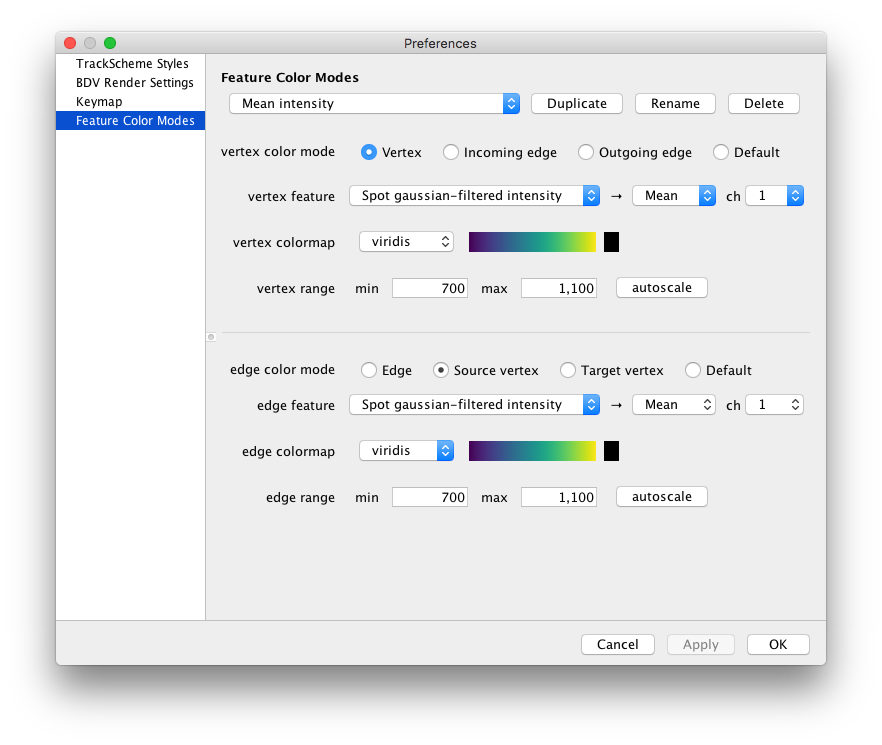
\includegraphics[height=0.3\textheight]{figures/Mastodon_FeatureColorModeConfig_2.png}
    
    \caption{Our custom feature color mode, based on spot intensity. }
    \label{fig:FeatureColorModeConfig2}
\end{figure}

Like for tag-sets, the \menu{View > Coloring} menu is now updated with items corresponding to the color modes we created.
If they are grayed-out, it means that the feature values they depend on is not yet computed.
This kind of view immediately reveals important aspect of the data, even at a very high level.
For instance with our custom color mode, we can quickly find cells that are the brightest, and visually inspect how the intensity in cells change over time (Figure~\ref{fig:FeatureColorModeView}).

\begin{figure}
    \centering
    \null\hfill
    \includegraphics[height=0.23\textheight]{figures/Mastodon_FeatureColorBDV.png}
    \hfill
    \includegraphics[height=0.23\textheight]{figures/Mastodon_FeatureColorTrackScheme.png}
    \hfill\null
    
    \caption{Feature color mode in a BDV view and in a \TrackScheme view.  }
    \label{fig:FeatureColorModeView}
\end{figure}


\subsection{Tags, numerical features and saving the data to disk.}

All tags and feature values are saved in the Mastodon file. 
The feature update stack state is saved too, so you will retrieve everything back as it was when you saved.
We did not have a choice, it was the only reasonable way to achieve a usable feature and tag framework in the case of very large data.


\subsection{The data table views.}
\label{sec:DataTables}

\subsubsection{The main table view.}

The BDV and \TrackScheme views are not suitable to display all the feature values we computed.
The coloring we have been using with them is good only for visualization purpose. 
There is a nice view to properly inspect and exploit feature values in subsequent steps in your analysis: the table view.
In practice, the table view is simply a tabular representation of the data items in Mastodon.
Spots and links are displayed in a list where a single row corresponds to a data item, and columns to feature values and tags. 
You can create a new table view by using the menu \menu{Window > New data table}.
If you did not compute features and did not define and tag-set, it should look like the table in figure~\ref{fig:TableViewEmpty}.
The view is made of two tables, one for spots (\texttt{Vertices} pane) and one for links (\texttt{Edges} pane).
Right now it is pretty empty. 
The spot and link tables only show the label and ID of the spots.
Navigating in this table is done classically: the arrow keys \menu{\arrowkeyup} and \keys{\arrowkeydown} jump from one row to the next, and \keys{\arrowkeyleft} and \keys{\arrowkeyright} from one column to the next.
\keys{Page\ \arrowkeyup} and \keys{Page\ \arrowkeydown} jump page per page.
\keys{\ctrl + Page\ \arrowkeyup} and \keys{\ctrl + Page\ \arrowkeydown} alternate between the spot table and the link table.

\begin{figure}
    \centering
    \null\hfill
    \includegraphics[height=0.23\textheight]{figures/Mastodon_TableView1.png}
    \hfill
    \includegraphics[height=0.23\textheight]{figures/Mastodon_TableView2.png}
    \hfill\null
    
    \caption{The table view, with no features computed and no tags defined. Left: the table for spots (\texttt{Vertices} pane). Right: the table for links (\texttt{Edges} pane).  }
    \label{fig:TableViewEmpty}
\end{figure}

After computing some features and defining some tag-sets, the table show new columns (Fi\-gu\-re~\ref{fig:TableViewFeatureTags}). 
Note that the column headers represent the feature with their projection and physical units on several rows.
For instance, the \texttt{Spot gaussian-filtered intensity} feature name is displayed on the first row of the column header.
The header is split in two columns on the second row, one for each projection included in the feature (mean and standard deviation of a single channel).
And in the third and last row, the units of each projection is display in brackets (Counts in this case).
The header of the tag-set columns are similar.
The first row shows the name of the tag-set, and the second row shows each of the tag the set contains, with the tag chosen color as background.

\begin{figure}
    \centering
    \includegraphics[height=0.27\textheight]{figures/Mastodon_TableView3.png}
    
    \caption{The table view, with features and tags.  }
    \label{fig:TableViewFeatureTags}
\end{figure}

The table view can be used to edit in part the data  (Fi\-gu\-re~\ref{fig:TableViewEditing}). 
For instance you can edit the spot label directly in the table. 
Just navigate to the row of spot you want to change the name of and the \texttt{Label} column, then press \keys{F2}.
The label field becomes editable.
When you are done editing, press \keys{\return}.
The tags are displayed as check-boxes in the table, that you can set directly by clicking on them.
Or you can navigate the desired row and column and set them with the \keys{Space} key.

\begin{figure}
    \centering
    \includegraphics[height=0.27\textheight]{figures/Mastodon_TableView4.png}
    
    \caption{After editing spot labels and tags.  }
    \label{fig:TableViewEditing}
\end{figure}

The highlight and selection are also shared with table views. 
When the table view is not active, selected items are shown with a gray background.
The highlight spot or link is shown in the table with a thick black border (Figure~\ref{fig:TableViewHighlightSelection}).
To add rows to the selection, the default key-bindings are again standard.
Press \keys{\shift+Left-click} to add a range of rows to the selection from a rable view, or use \keys{\shift+\arrowkeyup} or \keys{\shift+\arrowkeydown} or \keys{\shift+Page\ \arrowkeyup} and \keys{\shift+Page\ \arrowkeydown}.
By pressing \keys{\ctrl+Left-click} or \keys{\cmd+Left-click} you can toggle single rows in and out of the selection.
Of course, all of the commands related to the selection we have seen before also apply to the table views (Table~\ref{tab:MastodonSelectionKeys} page~\pageref{tab:MastodonSelectionKeys}).


Another feature of data tables is that they can be made slave of a spatial context, like for \TrackScheme.
When another BDV view is active, you can select its name in the drop-down list on the top-right part of the table. 
Then the table only shows the data items that are currently displayed in the master BDV view.
The notion of spatial context is explained above (section~\ref{sec:SpatialContext} page~\pageref{sec:SpatialContext}).
See also the figure~\ref{fig:SpatialContext} page~\pageref{fig:SpatialContext}.

\begin{figure}
    \centering
    \null\hfill
    \includegraphics[height=0.23\textheight]{figures/Mastodon_TableView5.png}
    \hfill
    \includegraphics[height=0.23\textheight]{figures/Mastodon_TableView6.png}
    \hfill\null
    
    \caption{Highlight and selection in the table view.  }
    \label{fig:TableViewHighlightSelection}
\end{figure}

\subsubsection{Sorting rows.}

The table can be sorted by clicking on the header of the column you want to use for sorting. 
It works for labels, IDs, feature values and tags

\subsubsection{The selection table.}

There exists a variation of the table view, but that display only what is currently in the selection.
To display such a table, go to \menu{Window > New selection table} in the menu.
The selection table that appears only shows what is in the selection, and is constantly updated to reflect changes in the selection (Figure~\ref{fig:SelectionTable}).
You cannot use it to edit the selection like in the main table.
However the row you pick in this table will set the focus and highlight in other views.
Everything else applies to the selection table.

\begin{figure}
    \centering
    \null\hfill
    \includegraphics[height=0.23\textheight]{figures/Mastodon_TableView7.png}
    \hfill
    \includegraphics[height=0.23\textheight]{figures/Mastodon_TableView8.png}
    \hfill\null
    
    \caption{The selection table.  }
    \label{fig:SelectionTable}
\end{figure}

\subsubsection{Feature-based coloring in table views.}

Of course, feature based coloring works with the table views (Figure~\ref{fig:TableViewFeatureColoring}).
And it can give a pleasant display when combined with sorting rows by a feature column.


\begin{figure}
    \centering
    \includegraphics[height=0.27\textheight]{figures/Mastodon_TableView9.png}
    
    \caption{Feature-based coloring in table views.  }
    \label{fig:TableViewFeatureColoring}
\end{figure}

\subsubsection{Exporting table data.}

The data currently displayed in a table view can be exported to CSV.
When a table window is active, select the menu item \menu{File > Export to CSV}.
You will have to specify a saving location and a name.
But two CSV files will be produced: one for the spot table (appended with \texttt{-vertices.csv}) and one for the link table (appended with \texttt{-edges.csv})
Only the data currently displayed in the view are saved, and ordered as in the view. 
This means that if you call the \menu{File > Export to CSV} command from a selection table, only the current selection will be saved.


\begin{table}[!htbp]
    \centering
    
    \caption{Default navigation key-bindings for Mastodon-table views.}

    \begin{tabulary}{\textwidth}{L|J}
    
    \toprule
    \textbf{Action}                 & \textbf{Key}              
    \\ \midrule
    
    \multicolumn{2}{c}{\textit{Navigation.}}
    \\ \midrule
    
    Move from row to row             & \keys{\arrowkeyup} and \keys{\arrowkeyup}.
    \\ \midrule
    
    Move column to column            & \keys{\arrowkeyleft} and \keys{\arrowkeyright}.
    \\ \midrule

    Display the spot table / the link table            & \keys{\ctrl + Page\ \arrowkeydown} and \keys{\ctrl + Page\ \arrowkeyup}.
    \\ \midrule

    \multicolumn{2}{c}{\textit{Editing.}}
    \\ \midrule
    
    Edit spot label                & \keys{F2} when focus is in the label column.
    \\ \midrule

    Toggle tag                      & \keys{Space} when focus is in the desired tag column.
    \\ \midrule
    
    \multicolumn{2}{c}{\textit{Selecting.}}
    \\ \midrule
    
    Add next / previous row to selection        & \keys{\shift+\arrowkeyup} and \keys{\shift+\arrowkeydown}
    \\ \midrule

    Add range to selection        & \keys{\shift+Page\ \arrowkeyup} and \keys{\shift+Page\ \arrowkeydown} or \keys{\shift+Left-click} 
    \\ \midrule

    Toggle row into selection        & \keys{\ctrl+Left-click} or \keys{\cmd+Left-click} 
    \\ \bottomrule

\end{tabulary}


    \label{tab:MastodonTableKeys}
    \vspace{-10pt}

\end{table}


% Feature, tags and tables.
\newpage
\section{Semi-automated tracking.}

Let us suppose we are dealing with a difficult image in which me must track only a subset of cells. 
The cells are difficult to track automatically, for instance because there are many spurious structures labelled. 
Or because there are other cells of different sizes in the tissue we are studying. 
Or because the image quality varies in time and space. 
The data is such that that fully automated algorithms introduced in chapter~\ref{sec:GettingStarted} won't give us fully accurate results. 
We can use the manual editing tools introduced in chapter~\ref{sec:ManuelEditing} and curate the results of automated tracking, manually removing spurious detections and links, and fixing incorrect ones. 
Another approach would be to start from a blank annotation and track manually only the cells we are interested in. 
Both approaches might be long and tedious. 
We introduce in this chapter tools for semi-automated tracking, that should alleviate the work of the second approach.

Semi-automated tracking is simply a way of following a specific cell that you picked-up manually. 
The tracker will follow the cell over time, and create spots and links for a certain amount of time-points.
It searches for the best spot candidate in the next time-point around the location of the spot.
It then creates a new spot there and links it to the previous one.
This procedure is repeated this for a certain number of time-points you can set, creating or augmenting a track starting from the spot you selected.

The semi-auto tracker can be configured to work backward in time (backtracking), to have a certain search radius, or a certain sensitivity to spot quality (as defined in chapter~\ref{sec:DetectingCells}).
The way it interacts with existing annotation can be configured too. 
You can make it stops when it meets an existing spot, linking to it or not.
You can make it connect to small tracks and resume tracking when it meets the track end.
You can force it to only create links on already existing spots. 
These configuration options give rise to several use-cases we will also survey in this chapter.
But the important message is that semi-automated tracking is a convenient means for dealing with difficult cases, when a fully automated approach fails, and when the data to track is large that doing it manually is inconvenient.
Or when you only care for a subset of cells in a dense tissue.

\subsection{Simple semi-automated tracking.}

We will introduce semi-automated tracking on a movie with empty annotation. 
Open the dataset we have been using so far, and clear all annotations (for instance select all \keys{\ctrl+A} then delete selection \keys{\shift+\backdel}).
Then pick a cell in the top layer, and create a spot, centered on its brightest part, like for instance on Figure~\ref{fig:BeforeSemiAutoTracking}.
Adjust its radius and select it.
Open a \TrackScheme window to visualize the tracking progress.

\begin{figure}
    \centering
    \null\hfill
    \includegraphics[width=0.3\textwidth]{figures/Mastodon_SemiAutoTracking_01a.png}
    \hfill
    \includegraphics[width=0.3\textwidth]{figures/Mastodon_SemiAutoTracking_01b.png}
    \hfill\null
    \caption{Manually picking a cell for semi-automated tracking.}
    \label{fig:BeforeSemiAutoTracking}
\end{figure}

To start semi-automated tracking, press \keys{\ctrl+T}.
A log window should open, and tracking should proceed. 
If the log does not complain about candidates being too far, you should end up with something resembling Figure~\ref{fig:AfterSemiAutoTracking}.
The tracking stopped after 10 frames, and the last spot added is now in the selection. 
Each spot is centered on the cell we started with, and it has the same radius that of the first spot we created. 
You can resume semi-automated tracking from the last spot created by just pressing \keys{\ctrl+T} again. 
If you do it one more time you should reach the end of the movie, with a new track following a single cell over the full movie duration.
To get it, you just had to press \keys{\ctrl+T} 3 times.
If you have more than one cell in the selection, they will be tracked one after another.

\begin{figure}
    \centering
    \null\hfill
    \includegraphics[width=0.2\textwidth]{figures/Mastodon_SemiAutoTracking_02.png}
    \hfill
    \includegraphics[width=0.4\textwidth]{figures/Mastodon_SemiAutoTracking_03.png}
    \hfill\null
    \caption{Results of semi-automated tracking.}
    \label{fig:AfterSemiAutoTracking}
\end{figure}


\subsection{Configuring the semi-automated tracker.}

\begin{figure}
    \centering
    \includegraphics[width=0.4\textwidth]{figures/Mastodon_SemiAutoTracking_04.png}
    \caption{The semi-automated tracking configuration panel.}
    \label{fig:ConfigSemiAutoTracking}
\end{figure}

The tracking does not always succeed. 
Depending on where you position the initial spot, it might fail, for instance stating in the log that if found a suitable spot, but outside the tolerance radius.
(In this example movie, this happens often because the cells are very elongated along the Z direction, and the tracker tends to find candidates near the top, brightest part of the cell.) 
The parameters that control for instance the tracker search radius can be set in the semi-automated tracking configuration dialog, in the \menu{Plugins > Tracking > Configure semi-automatic tracker}.
The window show in Figure~\ref{fig:ConfigSemiAutoTracking} should appear.
This dialog is very similar to the one used to configure feature color modes, that we have seen in chapter~\ref{sec:ConfigureColorModes} page~\pageref{sec:ConfigureColorModes}.
It also works the same way: the top elements are made to manage several tracking configuration, that will be stored on disk and retrieved in your next Mastodon session. 
There are two default tracking configuration: the \textbf{Forward} one is the default that we just used. 
The \textbf{Backtracking} configuration tracks backward in time. 
The other parameters controls the tracker behavior for the configuration currently selected in the top drop-down list.
To explain what they do we need first to describe how the semi-automated tracker works (Figure~\ref{fig:ExplainSemiAutoTracking}).

\begin{figure}
    \centering
    \includegraphics[width=0.45\textwidth]{figures/Mastodon_ExplainSemiAutoTracker_copie.pdf}
    \caption{Illustration of the semi-automated tracking process.}
    \label{fig:ExplainSemiAutoTracking}
\end{figure}

The semi-automated tracker works by processing only a small neighborhood around the initial spot, (called the \textit{source} spot later).
This neighborhood is centered on the spot center (in magenta in Figure~\ref{fig:ExplainSemiAutoTracking}), but taken in the next time-point (or previous one if you choose to go backward in time).
It applies the DoG detector (described in chapter~\ref{sec:DetectingCells} page~\pageref{sec:DetectingCells}) on this neighborhood, which yields several detections (green circles).
The detections that are found outside of a search radius (white, dashed circle) are not considered.
Detections inside the search radius but with a low quality are discarded as well.
The tracker therefore select the detection with a sufficiently large quality inside the search radius. 
If there is more than one suitable detection, it selects the one with the highest quality.
A new spot is created at this location, with the same radius that of the source spot. 
If the source spot is not a sphere but an ellipsoid, the smallest radius of the ellipsoid is taken. 
The newly created spot is then linked to the source spot. 
This is then repeated for the next time-point (or previous one), using the new spot as initial spot in the same process.
If no suitable detections are found within the search radius, the tracker stops, and the reason is printed in the tracker log window.

The configuration panel controls the parameters of this process.
\begin{itemize}
    
    \item \texttt{Setup ID} specifies what channel (or setup in case you have a multi-view dataset) that will be used for the detection.
    
    \item \texttt{Quality factor} specifies the threshold on quality below which we reject detections. This threshold is expressed in fraction of the source spot quality. For instance if the source spot quality is 60 and the \texttt{Quality factor} is 0.5, detections with a quality lower than 30 will rejected. If the source spot has no quality value (it was added manually), this parameter is ignored and all quality values are accepted.
    
    \item \texttt{Distance factor} specifies the search radius, in units of the source spot radius. For instance, for a value of 2.5, only detections that are within 2.5 \texttimes\, the radius of the source spot will be considered. Again, if the source spot is not a sphere but an ellipsoid, the smallest radius of the ellipsoid is taken. 
    
    \item \texttt{N time-points} specifies the number of time-points after which to stop.
    
    \item \texttt{Tracking direction} lets you specify whether you want tracking to happen forward or backward in time.
    
\end{itemize}

\noindent If you see that the tracker often stops with a message stating that it could not find a suitable candidate within search radius, try to either decrease  the value of the \texttt{Quality factor} or increase the value of the \texttt{Distance factor}.

\subsection{Tracker behavior with existing annotations.}

The next parameters below the \textbf{Existing spots} category configure how the tracker deals with existing annotations.
They change the behavior described in the previous section.
Indeed, before running the DoG detector on the neighborhood, the tracker first searches for an existing spot within the search radius. 
If it finds one, it does not run the DoG detection, but links to the existing spot (called \textit{target} spot later) or not, depending on the following parameters.

If the \texttt{Allow linking to an existing spot} checkbox is deselected, the tracker stops. 
If it is selected, the tracker will link to the target spot, provided it has no links already. 
However, the next 3 parameters allow to add exceptions: 

\begin{itemize}
    \item \texttt{Link even if target has incoming links}
    \item \texttt{Link even if target has outgoing links}
    \item \texttt{Continue tracking if source and target spots are already linked}
\end{itemize}

\noindent Their selection have important consequences when you are tracking along existing spots.
They are best exemplified by several different use-cases.

\subsection{Main use-cases for semi-automated tracking.}

\subsubsection{Tracking a subset of cells. }

This is what we have been doing in the first section of this chapter. 
This does not require any special configuration and the default tracking configuration called \textbf{Forward} will do.
Here is an example of when this use-case can be useful.

Arianne Bercowski Rama and Laurel Ann Rohde (Segmentation Timing and Dynamics Laboratory, EPFL) are studying the somatogenesis dynamics in the zebrafish embryo.
They acquire long-term time-lapse movies of the development of an embryo, with cellular resolution.
For this project they wanted to follow a few cells of interest (a few dozens per movie) and investigate the expression of a gene reporter as the cells moved along the zebrafish embryo.
The nuclei are all stained with a nuclear marker, so this fluorescence channel could be used for automated detection, but there are thousands of cells.
Instead, they relied on semi-automated tracking, selecting a the cells of interest in the first frames of the movie, and tracking them to the end thanks to the semi-automated tracker (Figure~\ref{fig:ArianneUseCase}, left). 
Once the tracking was done, they used feature analysis to extract fluorescence intensity over time for each cell in the gene reporter channel (Figure~\ref{fig:ArianneUseCase}, right).


\begin{figure}
    \centering
    \null\hfill
    \includegraphics[width=0.4\textwidth]{figures/Mastodon_ArianneUseCase_01.png}
    \hfill
    \includegraphics[width=0.4\textwidth]{figures/Mastodon_ArianneUseCase_02.png}
    \hfill\null
    \caption{Semi-automated tracking of a subset of cells during somatogenesis in the zebrafish embryo. \textbf{Left}: Image data overlaid with the tracks of the cells of interest. \textbf{Right}: Gene reporter fluorescence intensity for 10 of these cells as a function of time.}
    \label{fig:ArianneUseCase}
\end{figure}


\subsubsection{Stitching small track segments.}

The semi-automated tracker can be used with the same configuration to stitch small track segments, which follow the same cell but are separated and spread in time. 
This might be caused linking with missing detections, and the situation could resemble what is pictured in Figure~\ref{fig:Tracklets}.

We can use the semi-automated tracker to connect them, and add the missing detections.
We want the tracker to create spots for the cell in time-points when they are missing, and to connect to existing ones it will find by following the cell.
To allow this, we must enable first the '\texttt{Link even if target has outgoing links}' setting, so that the tracker does not stop when it meets a spot that is at the beginning of a track segment.
Second, we must enable the '\texttt{Continue tracking if source and target spots are already linked}' setting.
If we do not, the tracker will stop after connecting the first track segment it meets. 
Finally, we have to increase the value of the '\texttt{N time-points}' parameter, so that the tracker iterate through the full movie. 
After doing this and tracking for the first cell, we get a single track (Figure~\ref{fig:StitchedTracklets}).

\begin{figure}
    \centering
    \null\hfill
    \includegraphics[height=0.2\textheight]{figures/Mastodon_Tracklets_01.png}
    \hfill
    \includegraphics[height=0.2\textheight]{figures/Mastodon_Tracklets_02.png}
    \hfill\null
    \caption{Small discontinuous track segments following a single cell.}
    \label{fig:StitchedTracklets}
\end{figure}

\begin{figure}
    \centering
    \null\hfill
    \includegraphics[height=0.2\textheight]{figures/Mastodon_Tracklets_03.png}
    \hfill
    \includegraphics[height=0.2\textheight]{figures/Mastodon_Tracklets_04.png}
    \hfill
    \includegraphics[height=0.2\textheight]{figures/Mastodon_Tracklets_05.png}
    \hfill\null
    \caption{Results of stitching the track segments with the semi-automated tracker. Notice the messages on the log window that state what the tracker did when it meets existing spots.}
    \label{fig:Tracklets}
\end{figure}

\subsubsection{Backtracking, branching on cell divisions. }

Backtracking is particularly useful when creating lineages of cells that divide often in the movie.
Another application is in mapping differentiated cells at a late time-point, to the position of their progenitors at the beginning of the movie. 
For this we typically starts from an empty annotation, select a cell of interest in a late time-point, and backtrack it to its position in the beginning of the movie.
The built-in configuration called \textbf{Backtracking} is made for this.
If the cell we backtrack divided several times during the movie, might be creating tracks for sibling cells.
We want these tracks to branch properly in case we meet the mother cell when it divides.

This is why we need to enable the '\texttt{Link even if target has outgoing links}' setting, but no other.
Suppose we already have one track for a cell that divides, following the mother cell then one of the daughter cells. 
When we will backtrack from the other daughter cell, late in the movie, we will meet the division point of the mother cell. 
There is an existing spot there, just before the cell divides. 
It has already an outgoing link (to the first daughter we already tracked), and we want to connect to it. 
Hence we enable the '\texttt{Link even if target has outgoing links}' setting.
Because we want to stop tracking there (the rest of the track is good already), we do not enable any of the two other settings.



\subsubsection{Sparse linking over dense spots.}


% Semi automated-tracking.
\newpage
\section{The selection creator.}
\label{sec:SelectionCreator}

The automated detection process we use often generates a lot of spurious detections.
In TrackMate~\cite{TrackMate} we complemented it by adding \textit{feature filters} just after the detection step.
In TrackMate UI it takes the shape of filter windows, where the user can specify a feature and a threshold above or below which spots are rejected. 
The filters can be stacked to generate a more stringent filtering.
This approach is like fishing with a small-hole net, then throwing back unwanted fishes to sea.

In Mastodon we take a somewhat different approach.
We don't have a filter interface, but instead work with the selection tool.
To remove spurious spots, they are added to the selection based on criteria you define, then the selection content is deleted.
The tool to create a selection is called the selection creator and we describe it here. 
It works differently from the interactive selection we have been presenting before (see~\ref{sec:SelectionTool} page~\pageref{sec:SelectionTool} ).
Instead of manually clicking on spots or links, or drawing a selection rectangle in \TrackScheme, you will enter an expression that will be parsed to generate a selection.

We thought this approach would be more convenient and powerful.
First going through the selection allows to use the selection creator for other ends than filtering.
You can create a selection and assign a tag to it for instance (see~\ref{sec:AssigningTags} page~\pageref{sec:AssigningTags}).
Or use a selection as an input to the linking wizard (see~\ref{sec:SelectingInputForLinking} page~\pageref{sec:SelectingInputForLinking}).
Or have a BDV view that only shows the selection you just created (see~\ref{sec:BDVViewModes} page~\pageref{sec:BDVViewModes}).




\newpage
\part{Technical information.}
\vfill
\epigraph{
\textit{Frères humains qui après nous vivez \\ 
N'ayez les cœurs contre nous endurcis, \\
Car, se pitié de nous pauvres avez, \\ 
Dieu en aura plus tost de vous merciz.}
}{Francois Villon}

% The graph of Mastodon
\newpage
\section{The graph data structure of Mastodon.}

The \emph{mastodon-graph} Java package can be used to implement directed graphs with small memory footprint.
Vertices and edges are not stored as individual objects.
Instead vertex and edge data is laid out in a primitive \texttt{byte[]} array and accessed via proxy objects.
This chapter describes some internals of the \emph{trackmate-graph} package.

\pgfdeclarelayer{background}
\pgfsetlayers{background,main}

\tikzset{every picture/.append style={>=latex'}}

\tikzstyle{obj layout matrix}=[
  	matrix anchor=north west,
		inner sep=0pt,
		outer ysep=0pt,
		nodes={
			inner sep=3.5pt,
			draw,
			minimum height=7mm,
			text width=30mm,
			font=\ttfamily
		}
	]
	
\tikzstyle{obj layout indices}=[
  	matrix anchor=north east,
		xshift=4mm,
		nodes={
			%draw=gray!20,
			minimum height=7mm,
			text width=6mm,
			align=right,
			font=\ttfamily
		},
		text=blue
	]
	
\tikzstyle{edge layout indices}=[
		obj layout indices,
		text=red
	]
	
\tikzstyle{obj layout byte indices}=[
		obj layout indices,
		xshift=-2.5mm,
		yshift=2mm,
		text=gray
	]


% -------------------------------------
\subsection{Memory layout.}
% -------------------------------------

Each vertex and each edge maps to a contiguous portion of a \texttt{byte[]} array.
The size of a portion (\emph{elements}) is fixed for a particular \texttt{AbstractVertex} or \texttt{AbstractEdge} subclass.
Each \emph{element} starts with a fixed part that represents the graph structure and then additional payload used by the subclass to describe some vertex attributes, etc.
 
There is one \texttt{byte[]} array that stores all vertices, and one \texttt{byte[]} array that stores all edges.
References between these arrays are in the form of \emph{element indices}.
Whether these are indices refer to elements in the vertex or in the edge memory array is clear from the context.

% -------------------------------------
\subsubsection{Vertex layout.}
% ------------------------------------
The following diagram illustrates the layout of vertices in a \texttt{byte[]} array:
\begin{center}
	\begin{tikzpicture}[
			scale=0.8, every node/.style={scale=0.8},
			inner frame xsep=0mm,
			inner frame ysep=0mm,
			background rectangle/.style={
	    	fill=black!10
	    },
	    %show background rectangle
		]
		\newcommand{\spot}[4]{
		  \matrix (l) at (l.south west) [obj layout matrix]
		  {
		    \node (sl1) {FIRST\_IN\_EDGE}; \\
		    \node (sl2) {FIRST\_OUT\_EDGE}; \\
		    \node (sl3) [minimum height=20mm] {}; \\
		  };
		  
		  \draw
		  	[decoration={brace,amplitude=0.5em},decorate,thick]
		 			($(sl1.north east) + (3mm, -0.2mm)$) -- 
					($(sl2.south east) + (3mm, 0.2mm)$)
					node [anchor=west, midway, yshift=-1pt, xshift=2mm, font=\ttfamily] {AbstractVertex};
					
		  \draw
		  	[decoration={brace,amplitude=0.5em},decorate,thick]
		 			($(sl1.north east) + (1mm, -0.2mm)$) -- 
					($(sl3.south east) + (1mm, 0.2mm)$)
					node [anchor=west, midway, yshift=-1pt, xshift=2mm, font=\ttfamily] {Spot};
					
			\matrix (b) [obj layout byte indices]
			at (l.north west)
			{
		    \node {#2}; \\
		    \node {#3}; \\
		    \node {#4}; \\
			};
			\matrix (i) [obj layout indices]
			at (b.north west)
			{
		    \node {#1}; \\
			};
		}
		\coordinate (l);
		\spot{0}{0}{4}{8}
		\spot{1}{57}{61}{65}
	  \matrix (l) at (l.south west) [obj layout matrix]
	  {
	    \node (sl1) {FIRST\_IN\_EDGE}; \\
	    \node (sl2) [draw=none] {...}; \\
	  };
	  \draw (sl2.north west) -- (sl2.south west);
	  \draw (sl2.north east) -- (sl2.south east);
	  \draw (sl2.north west) -- (sl2.north east);
		\matrix (b) [obj layout byte indices]
		at (l.north west)
		{
	    \node {114}; \\
		};
		\matrix (i) [obj layout indices]
		at (b.north west)
		{
	    \node {2}; \\
		};
	\end{tikzpicture}
\end{center}
\noindent
In the left-most column, \emph{element indices} are shown (in blue), followed by byte indices (in grey).
In the example, each element of the \texttt{AbstractVertex} subclass \texttt{Spot} requires $57$ bytes to store.
The data for the $i$th \texttt{Spot} starts at byte $i \cdot 57$.
The fixed \texttt{AbstractVertex} part comprises element indices \texttt{FIRST\_IN\_EDGE} and \texttt{FIRST\_OUT\_EDGE}, occupying 4 bytes each.
The remaining 49 bytes are \texttt{Spot} attributes.

\texttt{FIRST\_IN\_EDGE} is the element index (in the edge memory array) of the first \emph{incoming} edge, i.e., an edge pointing to this vertex. The remaining incoming edges of the same vertex are stored as a linked list in the edge memory as described below.
If this vertex does not have any incoming edges \texttt{FIRST\_IN\_EDGE} is $-1$.

Similarly, \texttt{FIRST\_OUT\_EDGE} is the element index of the first \emph{outgoing} edge, i.e., an edge starting from this vertex. The remaining outgoing edges of the same vertex are stored as a linked list in the edge memory as described below.
If this vertex does not have any outgoing edges \texttt{FIRST\_OUT\_EDGE} is $-1$.

% -------------------------------------
\subsubsection{Edge layout.}
% -------------------------------------
The following diagram illustrates the layout of edges in a \texttt{byte[]} array:
\begin{center}
	\begin{tikzpicture}[
			scale=0.8, every node/.style={scale=0.8},
			inner frame xsep=0mm,
			inner frame ysep=0mm,
			background rectangle/.style={
	    	fill=black!10
	    },
	    %show background rectangle
		]
		\newcommand{\edge}[6]{
		  \matrix (l) at (l.south west) [obj layout matrix]
		  {
		    \node (sl1) {SOURCE}; \\
		    \node (sl2) {TARGET}; \\
		    \node (sl3) {NEXT\_SOURCE\_EDGE}; \\
		    \node (sl4) {NEXT\_TARGET\_EDGE}; \\
		    \node (sl5) [minimum height=12mm] {}; \\
		  };
		  
		  \draw
		  	[decoration={brace,amplitude=0.5em},decorate,thick]
		 			($(sl1.north east) + (3.5mm, -0.2mm)$) -- 
					($(sl4.south east) + (3.5mm, 0.2mm)$)
					node [anchor=west, midway, yshift=-1pt, xshift=2mm, font=\ttfamily] {AbstractEdge};
					
		  \draw
		  	[decoration={brace,amplitude=0.5em},decorate,thick]
		 			($(sl1.north east) + (1mm, -0.2mm)$) -- 
					($(sl5.south east) + (1mm, 0.2mm)$)
					node [anchor=west, midway, yshift=-1pt, xshift=3mm, font=\ttfamily] {Edge};
					
			\matrix (b) [obj layout byte indices]
			at (l.north west)
			{
		    \node {#2}; \\
		    \node {#3}; \\
		    \node {#4}; \\
		    \node {#5}; \\
		    \node {#6}; \\
			};
			\matrix (i) [edge layout indices]
			at (b.north west)
			{
		    \node {#1}; \\
			};
		}
		\coordinate (l);
		\edge{0} {0} {4} {8}{12}{16}
		\edge{1}{24}{28}{32}{36}{40}
	  \matrix (l) at (l.south west) [obj layout matrix]
	  {
	    \node (sl1) {SOURCE}; \\
	    \node (sl2) [draw=none] {...}; \\
	  };
	  \draw (sl2.north west) -- (sl2.south west);
	  \draw (sl2.north east) -- (sl2.south east);
	  \draw (sl2.north west) -- (sl2.north east);
		\matrix (b) [obj layout byte indices]
		at (l.north west)
		{
	    \node {48}; \\
		};
		\matrix (i) [edge layout indices]
		at (b.north west)
		{
	    \node {2}; \\
		};
	\end{tikzpicture}
\end{center}
\noindent
In the left-most column, \emph{element indices} are shown (in red), followed by byte indices (in grey).
In the example, each element of the \texttt{AbstractEdge} subclass \texttt{Edge} requires $24$ bytes to store.
The data for the $i$th \texttt{Edge} starts at byte $i \cdot 24$.
The fixed \texttt{AbstractEdge} part comprises element indices
	\texttt{SOURCE},
	\texttt{TARGET},
	\texttt{NEXT\_SOURCE\_EDGE}, and
	\texttt{NEXT\_TARGET\_EDGE}, occupying 4 bytes each.
The remaining 8 bytes are \texttt{Edge} attributes.

\texttt{SOURCE} is the element index (in the vertex memory array) of the vertex from which this edge starts.

\texttt{TARGET} is the element index (in the vertex memory array) of the vertex to which this edge points.

\texttt{NEXT\_SOURCE\_EDGE} is the element index (in the edge memory array) of the next outgoing edge of the source vertex,
	i.e., the next edge that has the same \texttt{SOURCE}.
If there is no such edge then \texttt{NEXT\_SOURCE\_EDGE} is $-1$.

\texttt{NEXT\_TARGET\_EDGE} is the element index (in the edge memory array) of the next incoming edge of the target vertex,
	i.e., the next edge that has the same \texttt{TARGET}.
If there is no such edge then \texttt{NEXT\_TARGET\_EDGE} is $-1$.





% -------------------------------------
\subsubsection{Example}
% -------------------------------------

\tikzstyle{spot matrix}=[
  	matrix anchor=north west,
		inner sep=0pt,
		outer ysep=0pt,
		nodes={
			inner sep=3.5pt,
			draw,
			minimum height=5mm,
			text width=9mm,
			align=right,
		}
	]

\tikzstyle{incoming edge}=[
		green!50!black,
		thick,
		->,
		shorten >=1mm,
		shorten <=1mm,
		text=green!50!black,
		anchor=east
	]

\tikzstyle{outgoing edge}=[
		orange!70!black,
		thick,
		->,
		shorten >=1mm,
		shorten <=1mm,
		text=orange!50!black,
		anchor=east
	]

\tikzstyle{incoming bg}=[
		fill=green!10,
		inner sep=0pt
	]

\tikzstyle{outgoing bg}=[
		fill=orange!10,
		inner sep=0pt
	]

\newcommand{\spot}[4]{
  \matrix (s) at (s.south west) [spot matrix]
  {
    \node (s#4c1) [text=red] {#1}; \\
    \node (s#4c2) [text=red] {#2}; \\
    \node (s#4c3) [minimum height=13.5mm] {}; \\
  };
	\node at (s#4c1.west) [text width=2mm, draw=none, xshift=2mm, text=black] {$#4$};
	\node at (s#4c1.west) [text width=3mm, draw=none, xshift=-1mm, text=blue, font=\scriptsize] {#3};
}

\newcommand{\edge}[6]{
  \matrix (e) at (e.south west) [spot matrix]
  {
  	\node (e#6c1) [text=blue] {#1}; \\
    \node (e#6c2) [text=blue] {#2}; \\
    \node (e#6c3) [text=red]  {#3}; \\
    \node (e#6c4) [text=red]  {#4}; \\
    \node (e#6c5) [minimum height=9mm] {}; \\
  };
	\node at (e#6c1.west) [text width=2mm, draw=none, xshift=2mm, text=black] {$#6$};
	\node at (e#6c1.west) [text width=3mm, draw=none, xshift=-1mm, text=red, font=\scriptsize] {#5};
}

Consider the following example graph comprising vertices $A, B, C, D, E$ and edges $a, b, c, d$.
\begin{center}
	\tikzstyle{spot node}=[
			circle,
			very thick,
			draw=blue,
			text=blue,
			edge from parent/.style={red,draw},
		]
	\tikzstyle{edge link}=[
			text=red
		]
	
	\begin{tikzpicture}[
			level distance=14mm,
	    edge from parent/.style={red,very thick,draw},
			->]
	  \node [spot node] {$A$}
	  child {
			node [spot node] {$B$}
		  child [level distance=10mm, sibling distance=25mm ] {
				node [spot node] {$C$}
				edge from parent node [above left] {$b$}
			}
		  child [level distance=10mm, sibling distance=25mm ] {
				node [spot node] {$D$}
			  child [level distance=14mm] {
					node [spot node] {$E$}
					edge from parent node [edge link, right] {$d$}
				}
				edge from parent node [above right] {$c$}
			}
			edge from parent node [right] {$a$}
		};
	\end{tikzpicture}
\end{center}
This is laid out in memory as follows
\begin{center}
	\begin{tikzpicture}
		\coordinate (s);
		\spot {$-1$}  {$0$}   {0}{A}
		\spot  {$0$}  {$1$}   {1}{B}
		\spot  {$1$} {$-1$}   {2}{C}
		\spot  {$2$}  {$3$}   {3}{D}
		\spot  {$3$} {$-1$}   {4}{E}
		
		\coordinate (e) at (5,0);
		\edge  {$0$}  {$1$} {$-1$} {$-1$}   {0}{a}
		\edge  {$1$}  {$2$}  {$2$} {$-1$}   {1}{b}
		\edge  {$1$}  {$3$} {$-1$} {$-1$}   {2}{c}
		\edge  {$3$}  {$4$} {$-1$} {$-1$}   {3}{d}
		
		\tikzstyle{edge loop}=[
			to path={.. controls +(180:1) and +(-200:1) .. (\tikztotarget) \tikztonodes}
		]
	    
	  \draw [incoming edge] (sBc1.east) to [out=0, in=180] ($(eac1.west)-(2mm,0mm)$);
	  \node [incoming edge] at (eac4.west) {$\bot$};

	  \draw [outgoing edge] (sBc2.east) to [out=0, in=180] ($(ebc1.west)-(2mm,0mm)$);
	  \draw [outgoing edge] (ebc3.west) to [edge loop] ($(ecc1.west)-(2mm,0mm)$);
	  \node [outgoing edge] at (ecc3.west) {$\bot$};

		\begin{pgfonlayer}{background}
	  	\node [incoming bg, fit=(sBc1)] {};
	  	\node [incoming bg, fit=(eac4)] {};
	  	\node [outgoing bg, fit=(sBc2)] {};
	  	\node [outgoing bg, fit=(ebc3)] {};
	  	\node [outgoing bg, fit=(ecc3)] {};
	  \end{pgfonlayer}
	\end{tikzpicture}
\end{center}
The links between vertex $B$ and it's adjacent edges $a, b, c$ have been highlighted.
Let's look at that in more detail:
Vertex $B$ is stored at element index $1$ in the vertex memory array.
$B$ has one incoming edge $a$.
The edge $a$ is stored at element index $0$ in the edge memory array.
Therefore the \texttt{FIRST\_IN\_EDGE} field of $B$ is $0$.
%
Apart from $a$, the vertex $B$ has no further incoming edges.
Therefore, the \texttt{NEXT\_TARGET\_EDGE} field of $a$ is $-1$, i.e., the list of edges entering $B$ terminates here.

$B$ has two outgoing edges $b, c$.
The edge $b$ is stored at element index $1$ in the edge memory array.
Therefore the \texttt{FIRST\_OUT\_EDGE} field of $B$ is $1$.
%
The next outgoing edge of $B$ is $c$ which is stored at element index $2$.
Therefore, the \texttt{NEXT\_SOURCE\_EDGE} field of $b$ is $2$.
After $c$, the vertex $B$ has no further outgoing edges.
Therefore, the \texttt{NEXT\_SOURCE\_EDGE} field of $c$ is $-1$, i.e., the list of edges leaving $B$ terminates here.

Below is the same memory layout again, this time highlighting the references from edges $a, b, c$ back to the vertex memory array.
\begin{center}
	\begin{tikzpicture}
		\coordinate (s);
		\spot {$-1$}  {$0$}   {0}{A}
		\spot  {$0$}  {$1$}   {1}{B}
		\spot  {$1$} {$-1$}   {2}{C}
		\spot  {$2$}  {$3$}   {3}{D}
		\spot  {$3$} {$-1$}   {4}{E}
		
		\coordinate (e) at (5,0);
		\edge  {$0$}  {$1$} {$-1$} {$-1$}   {0}{a}
		\edge  {$1$}  {$2$}  {$2$} {$-1$}   {1}{b}
		\edge  {$1$}  {$3$} {$-1$} {$-1$}   {2}{c}
		\edge  {$3$}  {$4$} {$-1$} {$-1$}   {3}{d}
		
	  \draw [outgoing edge] ($(eac1.west)-(2mm,0mm)$) to [out=180, in=0]   (sAc1.east);
	  \draw [incoming edge]   (eac2.west)             to [out=180, in=0] ($(sBc1.east)+(0mm,1mm)$);

	  \draw [outgoing edge] ($(ebc1.west)-(2mm,0mm)$) to [out=180, in=0]   (sBc1.east);
	  \draw [incoming edge]   (ebc2.west)             to [out=180, in=0]   (sCc1.east);

	  \draw [outgoing edge] ($(ecc1.west)-(2mm,0mm)$) to [out=180, in=0] ($(sBc1.east)-(0mm,1mm)$);
	  \draw [incoming edge]   (ecc2.west)             to [out=180, in=0]   (sDc1.east);
	\end{tikzpicture}
\end{center}
For example, edge $c$ is leaving vertex $B$ (index $1$) and entering vertex $D$ (index $3$).
Therefore the \texttt{SOURCE} field of $c$ is $1$, and the \texttt{TARGET} field of $c$ is $3$.





% -----------------------------------------
\subsection{Free-list of unallocated elements.}
% -----------------------------------------

\tikzstyle{free bg}=[
		fill=gray!20,
		inner sep=0pt
	]

\newcommand{\freespot}[2]{
  \matrix (s) at (s.south west) [spot matrix]
  {
    \node (s#2c1) {$\mathbf{-2}$}; \\
    \node (s#2c2) {#1}; \\
    \node (s#2c3) [minimum height=13.5mm] {}; \\
  };
	\node at (s#2c1.west) [text width=3mm, draw=none, xshift=-1mm, text=blue, font=\scriptsize] {#2};
	\begin{pgfonlayer}{background}
  	\node [free bg, fit=(s#2c1)(s#2c3)] {};
  \end{pgfonlayer}
}

\newcommand{\freeedge}[2]{
  \matrix (e) at (e.south west) [spot matrix]
  {
  	\node (e#2c1) {$\mathbf{-2}$}; \\
    \node (e#2c2) {#1}; \\
    \node (e#2c3) [minimum height=19mm] {}; \\
  };
	\node at (e#2c1.west) [text width=3mm, draw=none, xshift=-1mm, text=red, font=\scriptsize] {#2};
	\begin{pgfonlayer}{background}
  	\node [free bg, fit=(e#2c1)(e#2c3)] {};
  \end{pgfonlayer}
}


The vertex and edge memory arrays can only ever grow.
When elements are released, they are simply marked as free for re-use.
Assume that in the above example vertex $D$ is deleted, as well as it's adjacent edges $c, d$, leaving this:
\begin{center}
	\tikzstyle{spot node}=[
			circle,
			very thick,
			draw=blue,
			text=blue,
			edge from parent/.style={red,draw},
		]
	\tikzstyle{edge link}=[
			text=red
		]
	
	\begin{tikzpicture}[
			level distance=14mm,
	    edge from parent/.style={red,very thick,draw},
			->]
	  \node [spot node] {$A$}
	  child {
			node [spot node] {$B$}
		  child [level distance=10mm, sibling distance=25mm ] {
				node [spot node] {$C$}
				edge from parent node [above left] {$b$}
			}
		  child [level distance=10mm, sibling distance=25mm] {
				node [spot node, draw=gray!40, text=gray!40] {$D$}
			  child [level distance=14mm] {
					node [spot node] {$E$}
					edge from parent [draw=gray!40, text=gray!40] node [right] {$d$}
				}
				edge from parent [draw=gray!40, text=gray!40] node [above right] {$c$}
			}
			edge from parent node [right] {$a$}
		};
	\end{tikzpicture}
\end{center}

\noindent
After removing $c, d, D$ the memory layout looks like this:

\begin{center}
	\begin{tikzpicture}
		\coordinate (s);
		\spot {$-1$}  {$0$}   {0}{A}
		\spot  {$0$}  {$1$}   {1}{B}
		\spot  {$1$} {$-1$}   {2}{C}
		\freespot {$-1$} {3}
		\spot {$-1$} {$-1$}   {4}{E}
		
		\coordinate (e) at (5,0);
		\edge  {$0$}  {$1$} {$-1$} {$-1$}   {0}{a}
		\edge  {$1$}  {$2$} {$-1$} {$-1$}   {1}{b}
		\freeedge {$-1$} {2}
		\freeedge {$2$} {3}
		
		\tikzstyle{edge loop}=[
			to path={.. controls +(180:1.5) and +(-170:1.5) .. (\tikztotarget) \tikztonodes}
		]
		\tikzstyle{freed edge}=[
				black,
				thick,
				->,
				shorten >=1mm,
				shorten <=1mm,
				anchor=east
			]
	    
		\node [freed edge] (ffs) at ($(s3c1.west)-(10mm,0mm)$) {\texttt{free}};
	  \draw [freed edge, shorten <=0mm] (ffs) to ($(s3c1.west)-(2mm,0mm)$);
	  \node [freed edge] at (s3c2.west) {$\bot$};

		\node [freed edge] (ffe) at ($(e3c1.west)-(13mm,0mm)$) {\texttt{free}};
	  \draw [freed edge, shorten <=0mm] (ffe) to ($(e3c1.west)-(2mm,0mm)$);
	  \draw [freed edge] (e3c2.west) to [edge loop] ($(e2c1.west)-(2mm,0mm)$);
	  \node [freed edge] at (e2c2.west) {$\bot$};
	  
		\node [draw=none] at ($(e2c1.east)+(18mm,0mm)$) {};	  
	\end{tikzpicture}
\end{center}
The element $3$ in the vertex memory array as well as elements $2$ and $3$ in the edge memory array have been marked as free.
This is done by putting the magic number ``$-2$'' into the first 4 bytes of the element.\footnote{
	In vertices and edges the first 4 bytes are always occupied by a (positive) index or a $-1$ index list terminator.
	Therefore, occupied and free blocks can not be confused.}
The next 4 bytes of a freed element are the index of the next freed element in the (same) memory array,
	or $-1$ if there is no next freed element.
Each memory array remembers the index \texttt{free} of the first freed element.

Newly freed elements are enqueued at \texttt{free}, that is, at the head of the free-list.
So in the above example, edge element $2$ was freed first, followed by edge element $3$.

The next edge element will be allocated at head of the free-list and the \texttt{free} index move to the next element.
For example, assume that a new edge is created from $B$ to $E$:
\begin{center}
	\begin{tikzpicture}
		\coordinate (s);
		\spot {$-1$}  {$0$}   {0}{A}
		\spot  {$0$}  {$1$}   {1}{B}
		\spot  {$1$} {$-1$}   {2}{C}
		\freespot {$-1$} {3}
		\spot {$3$} {$-1$}   {4}{E}
		
		\coordinate (e) at (5,0);
		\edge  {$0$}  {$1$} {$-1$} {$-1$}   {0}{a}
		\edge  {$1$}  {$2$} {$3$} {$-1$}   {1}{b}
		\freeedge {$-1$} {2}
		\edge  {$1$}  {$4$} {$-1$} {$-1$}   {3}{ }
		
		\tikzstyle{edge loop}=[
			to path={.. controls +(180:1.5) and +(-170:1.5) .. (\tikztotarget) \tikztonodes}
		]
		\tikzstyle{freed edge}=[
				black,
				thick,
				->,
				shorten >=1mm,
				shorten <=1mm,
				anchor=east
			]
	    
		\node [freed edge] (ffs) at ($(s3c1.west)-(10mm,0mm)$) {\texttt{free}};
	  \draw [freed edge, shorten <=0mm] (ffs) to ($(s3c1.west)-(2mm,0mm)$);
	  \node [freed edge] at (s3c2.west) {$\bot$};

		\node [freed edge] (ffe) at ($(e2c1.west)-(13mm,0mm)$) {\texttt{free}};
	  \draw [freed edge, shorten <=0mm] (ffe) to ($(e2c1.west)-(2mm,0mm)$);
	  \node [freed edge] at (e2c2.west) {$\bot$};
	  
		\node [draw=none] at ($(e2c1.east)+(18mm,0mm)$) {};	  
	\end{tikzpicture}
\end{center}
If \texttt{free} is -1, then no more freed elements are available and the underlying memory array has to grow to fit newly added elements.






\newpage
\bibliographystyle{ieeetr}
\clearpage 
\bibliography{References}









\end{document}
% vim::set expandtab tabstop=4 softtabstop=2 shiftwidth=2 ft=tex:
